%!TEX TS-program = pdflatexmk
\documentclass[cleanfoot]{asme2ej}

\usepackage[]{graphicx}
\graphicspath{ {images/} }

\usepackage{enumitem}
\usepackage{amsmath,amssymb}
\usepackage{textcomp}
\usepackage[urlcolor=blue,linkcolor=red,colorlinks=true]{hyperref}
\usepackage[autostyle, english=american]{csquotes}
\MakeOuterQuote{"}

\title{Exoplanet Open-Source Imaging Mission Simulator (EXOSIMS) \\ Interface Control Document}

%%% first author
\author{Daniel Garrett and Dmitry Savransky
    \affiliation{
    Sibley School of Mechanical and Aerospace Engineering\\
	Cornell University\\
	Ithaca, NY 14853
    }	
}

\def\mf{\mathbf}
\def\mb{\mathbb}
\def\mc{\mathcal}
\newcommand{\R}{\mathbf{r}}
\newcommand{\bc}{\mathbf{b}}
\newcommand{\mfbar}[1]{\mf{\bar{#1}}}
\newcommand{\mfhat}[1]{\mf{\hat{#1}}}
\newcommand{\bmu}{\boldsymbol{\mu}}
\newcommand{\blam}{\boldsymbol{\Lambda}}
\newcommand{\refeq}[1]{Equation  (\ref{#1})} 
\newcommand{\reftable}[1]{Table \ref{#1}} 
\newcommand{\refch}[1]{Chapter  \ref{#1}} 
\newcommand{\reffig}[1]{Figure \ref{#1}}
\newcommand{\refcode}[1]{Listing \ref{#1}}
\newcommand{\intd}[1]{\ensuremath{\,\mathrm{d}#1}}
\newcommand{\leftexp}[2]{{\vphantom{#2}}^{#1}\!{#2}}
\newcommand{\leftsub}[2]{{\vphantom{#2}}_{#1}\!{#2}}
\newcommand{\fddt}[1]{\ensuremath{\leftexp{\mathcal{#1}}{\frac{\mathrm{d}}{\mathrm{d}t}}}}
\newcommand{\fdddt}[1]{\ensuremath{\leftexp{\mathcal{#1}}{\frac{\mathrm{d}^2}{\mathrm{d}t^2}}}}
\newcommand{\omegarot}[2]{\ensuremath{\leftexp{\mathcal{#1}}{\boldsymbol{\omega}}^{\mathcal{#2}}}}


\begin{document}

\maketitle    

%%%%%%%%%%%%%%%%%%%%%%%%%%%%%%%%%%%%%%%%%%%%%%%%%%%%%%%%%%%%%%%%%%%%%%
\begin{abstract}
{\it This document describes the extensible, modular, open source software framework EXOSIMS.  EXOSIMS creates end-to-end simulations of space-based exoplanet imaging missions using stand-alone software modules.  These modules are split into input and simulation module groups.  The input/output interfaces of each module and interactions of modules with each other are presented to give guidance on mission specific modifications to the EXOSIMS framework. Last Update: \today}
\end{abstract}

\tableofcontents

%%%%%%%%%%%%%%%%%%%%%%%%%%%%%%%%%%%%%%%%%%%%%%%%%%%%%%%%%%%%%%%%%%%%%%
\begin{nomenclature}
\entry{EXOSIMS}{Exoplanet Open-Source Imaging Mission Simulator}
\entry{ICD}{Interface Control Document}
\entry{MJD}{Modified Julian Day}
\end{nomenclature}

%%%%%%%%%%%%%%%%%%%%%%%%%%%%%%%%%%%%%%%%%%%%%%%%%%%%%%%%%%%%%%%%%%%%%%
% INTRODUCTION
%%%%%%%%%%%%%%%%%%%%%%%%%%%%%%%%%%%%%%%%%%%%%%%%%%%%%%%%%%%%%%%%%%%%%%

\section{Introduction} 
Building confidence in a mission concept's ability to achieve its science goals is always desirable.  Unfortunately, accurately modeling the science yield of an exoplanet imager can be almost as complicated as designing the mission.  It is challenging to compare science simulation results and systematically test the effects of changing one aspect of the instrument or mission design.

EXOSIMS (Exoplanet Open-Source Imaging Mission Simulator) addresses this problem by generating ensembles of mission simulations for exoplanet direct imaging missions to estimate science yields. It is designed to allow systematic exploration of exoplanet imaging mission science yields.  It consists of stand-alone modules written in Python which may be modified without requiring modifications to other portions of the code. This allows EXOSIMS to be easily used to investigate new designs for instruments, observatories, or overall mission designs independently. This document describes the required input/output interfaces for the stand-alone modules to enable this flexibility.

\subsection{Purpose and Scope} % Rework this section
This Interface Control Document (ICD) provides an overview of the software framework of EXOSIMS and some details on its component parts.  As the software is intended to be highly reconfigurable, operational aspects of the code are emphasized over implementational details.  Specific examples are taken from the coronagraphic instrument under development for WFIRST-AFTA.  The data inputs and outputs of each module are described. Following these guidelines will allow the code to be updated to accommodate new mission designs.

This ICD defines the input/output of each module and the interfaces between modules of the code.  This document is intended to guide mission planners and instrument designers in the development of specific modules for new mission designs.

%\subsection{Glossary}
%This section will contain definition of terms used throughout the document if needed.

\section{Overview}
The terminology used to describe the software implementation is loosely based upon object-oriented programing (OOP) terminology, as implemented by the Python language, in which EXOSIMS is built.  The term module can refer to the object class prototype representing the abstracted functionality of one piece of the software, an implementation of this object class which inherits the attributes and methods of the prototype, or an instance of this class.  Input/output definitions of modules refer to the class prototype.  Implemented modules refer to the inherited class definition.  Passing modules (or their outputs) means the instantiation of the inherited object class being used in a given simulation.  Relying on strict inheritance for all implemented module classes provides an automated error and consistency-checking mechanism.  The outputs of a given object instance may be compared to the outputs of the prototype.  It is trivial to pre-check whether a given module implementation will work within the larger framework, and this approach allows for flexibility and adaptability.

\begin{figure}[ht]
    \begin{center}
        \begin{tabular}{c}
             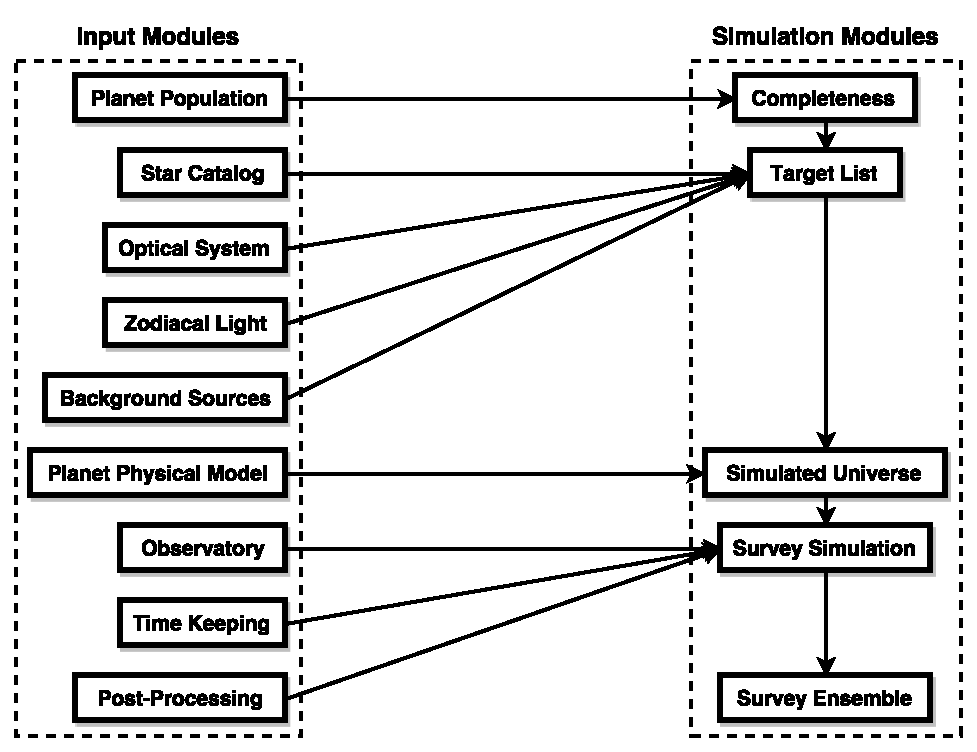
\includegraphics[width=0.9\textwidth]{codeflow5}
        \end{tabular}
    \end{center}
    \caption{EXOSIMS modules. Each box represents a component software module that interacts with other modules as indicated by the arrows. The simulation modules pass all input modules along with their own output.  Thus, the Survey Ensemble module has access to all of the input modules and all of the upstream simulation modules.}
    \label{figure_framework}
\end{figure}

The overall framework of EXOSIMS is depicted in \reffig{figure_framework} where the software components are classified as input modules and simulation modules.  The input modules include the Optical System, Star Catalog, Planet Population, Observatory, Planet Physical Model, Time Keeping, Zodiacal Light, Background Sources, and Post-Processing modules.  Objects of input module classes can be instantiated independently, without creating instances of any other module.  These modules contain specific mission design parameters and physical descriptions of the universe, and will change according to mission and planet population of interest.  The simulation modules include Target List, Simulated Universe, Survey Simulation, and Survey Ensemble modules.  The simulation modules take information contained in the input modules and perform mission simulation tasks. The instantiation of an object of any of these modules requires the instantiation of one or more input module objects (see \reffig{fig:instantiation_tree}).  Any module may perform any number or kind of calculations using any or all of the input parameters provided.  The specific implementations are only constrained by their input and output specification contained in this document.

\begin{figure}[ht]
    \begin{center}
        \begin{tabular}{c}
             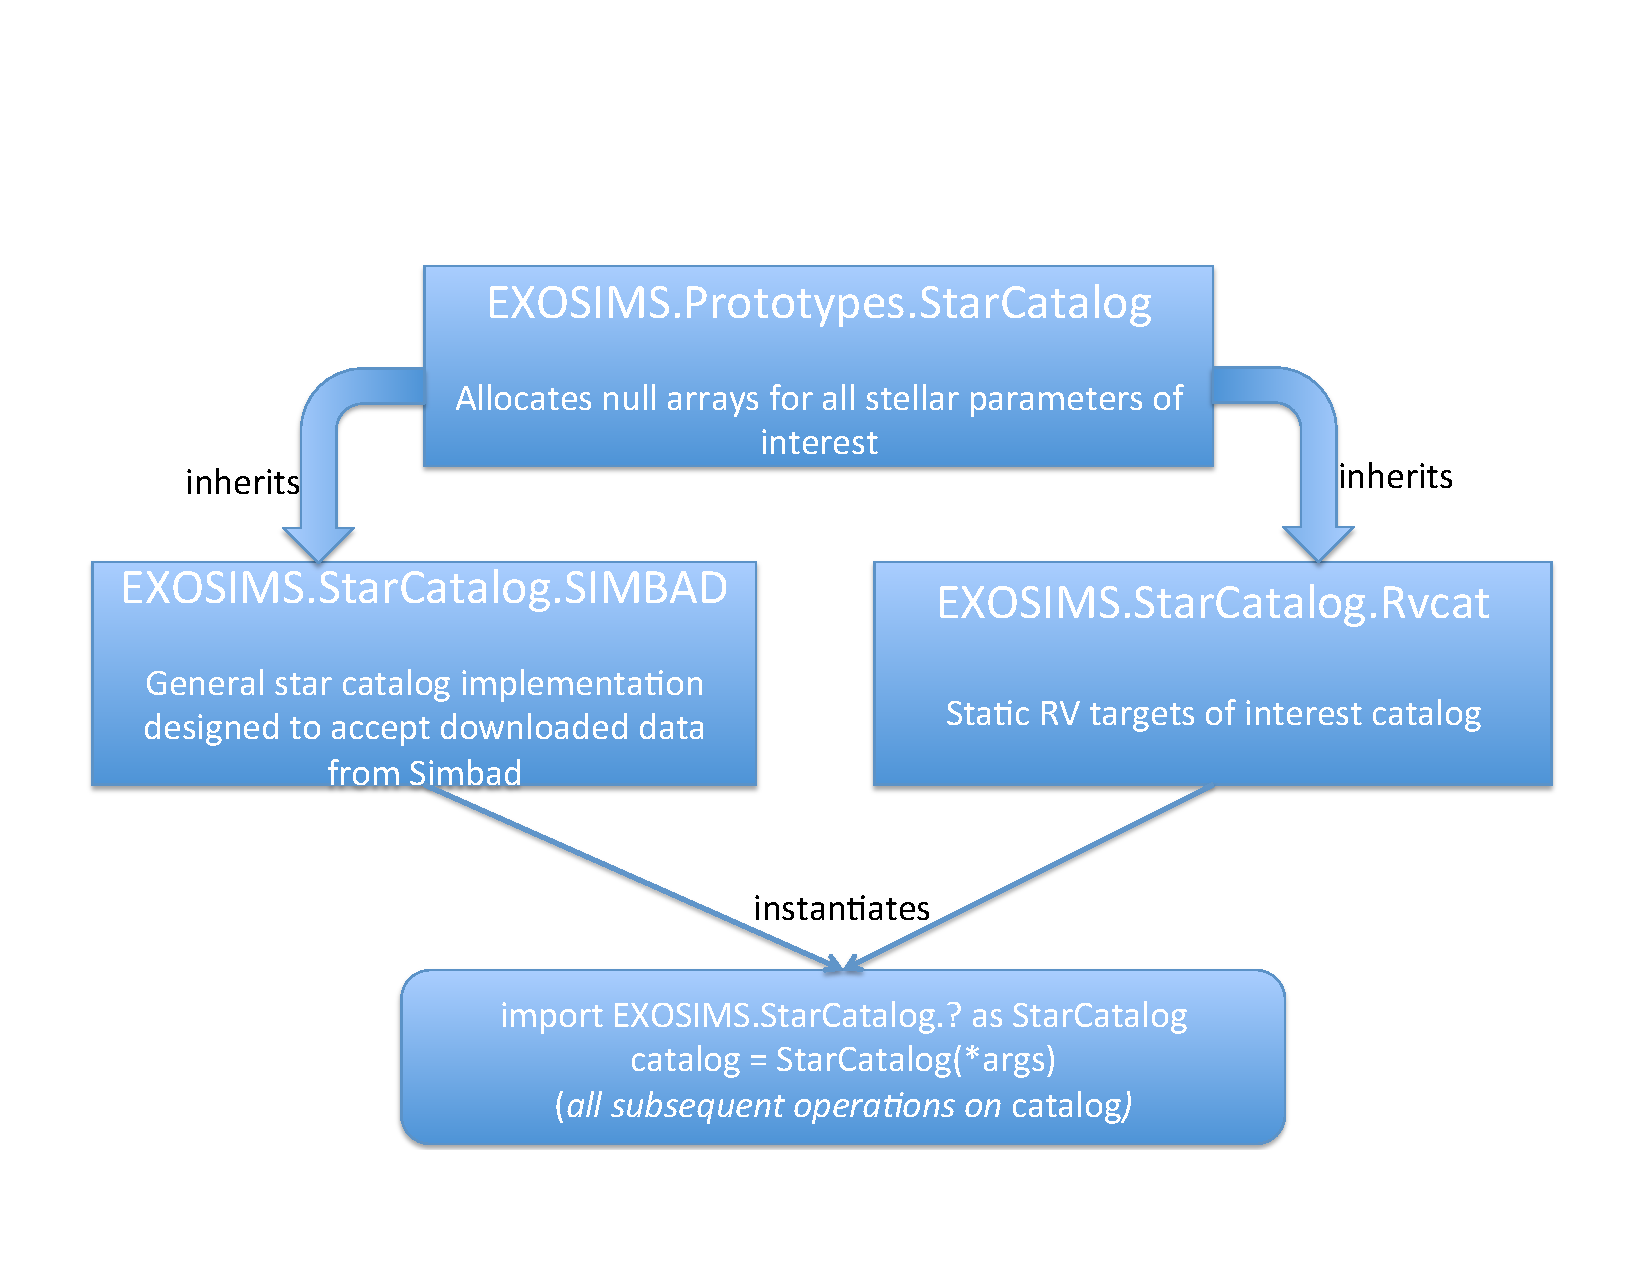
\includegraphics[width=0.75\textwidth]{starcatalog_flowdown}
        \end{tabular}
    \end{center}
    \caption{Schematic of a sample implementation for the three module layers for the Star Catalog module. The Star Catalog prototype (top row) is immutable, specifies the input/output structure of the module along with all common functionality, and is inherited by all Star Catalog class implementations (middle row).  In this case, two different catalog classes are shown: one that reads in data from a SIMBAD catalog dump, and one which contains only information about a subset of known radial velocity targets.  The object used in the simulation (bottom row) is an instance of one of these classes, and can be used in exactly the same way in the rest of the code due to the common input/output scheme.}
    \label{fig:starcatalog_flowdown}
\end{figure}

\begin{figure}[ht]
    \begin{center}
        \begin{tabular}{c}
             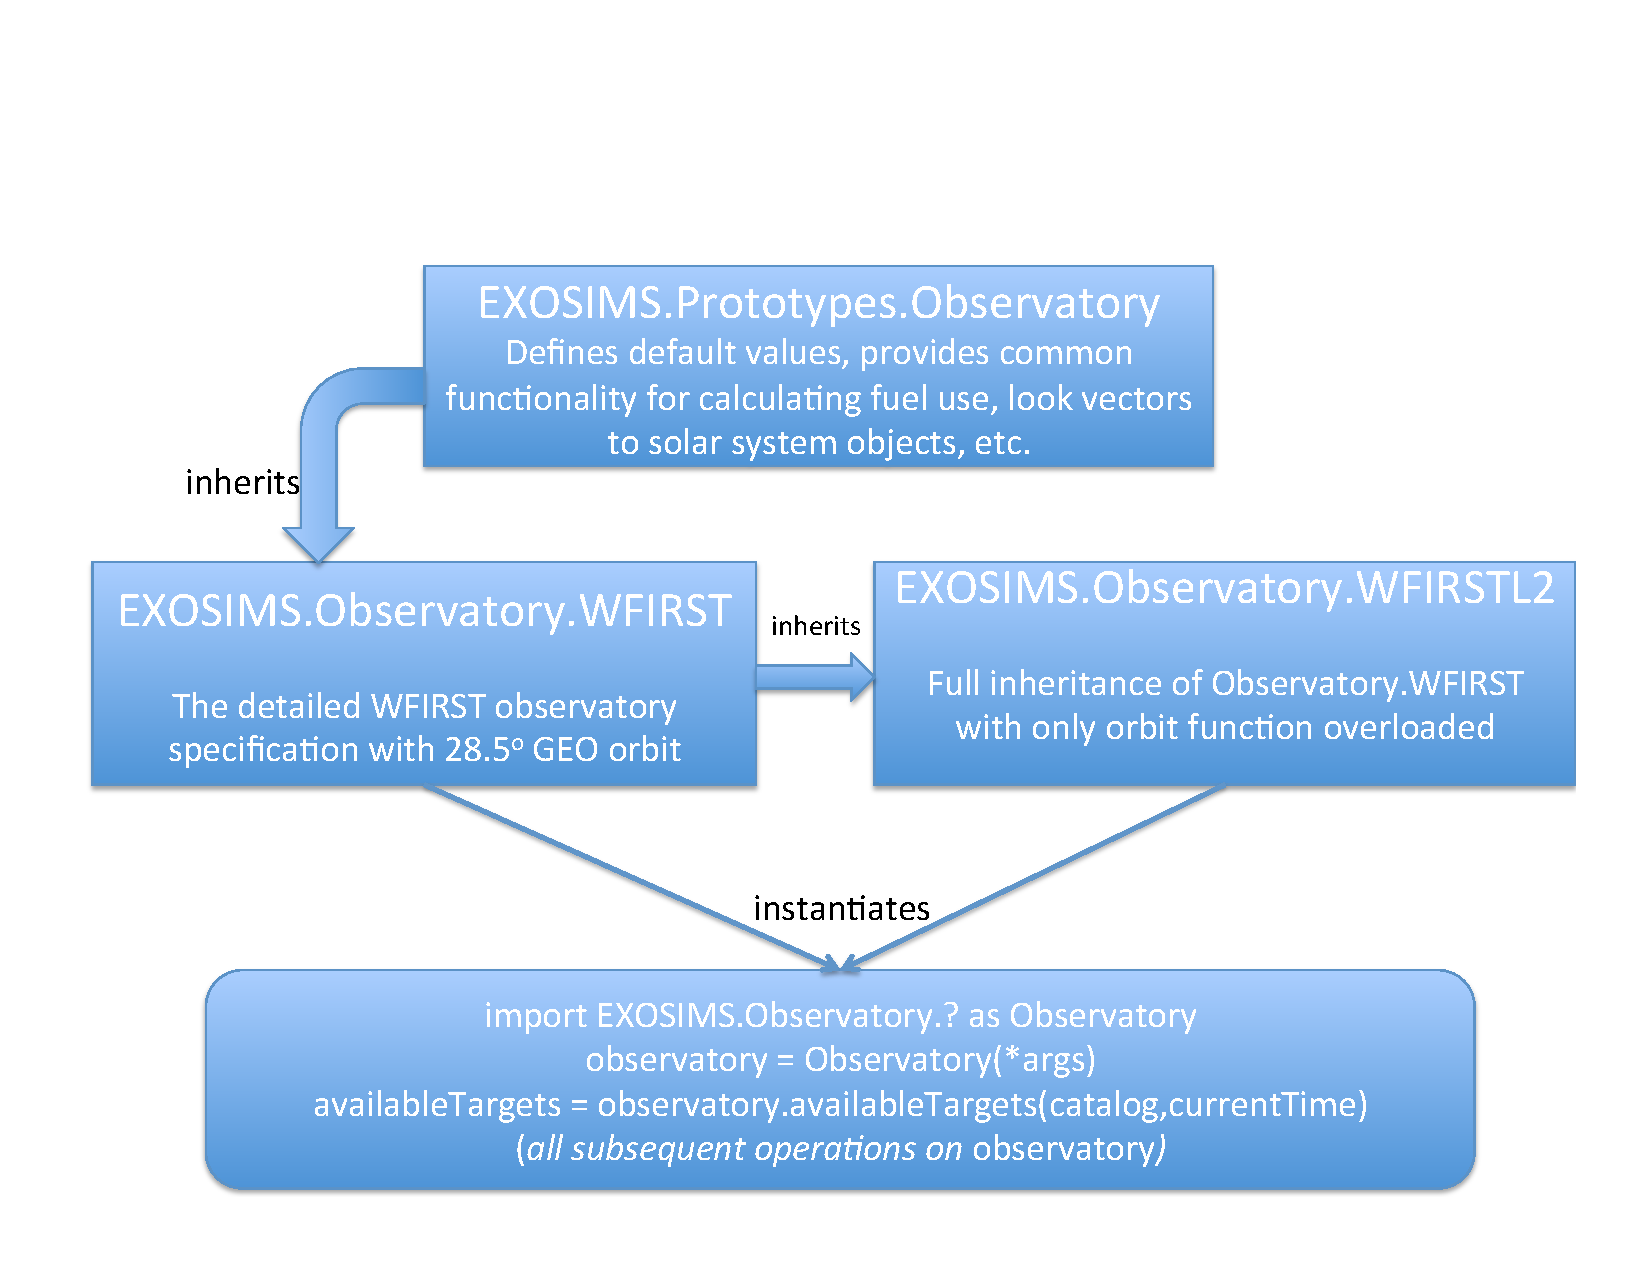
\includegraphics[width=0.75\textwidth]{observatory_flowdown}
        \end{tabular}
    \end{center}
    \caption{Schematic of a sample implementation for the three module layers for the Observatory module. The Observatory prototype (top row) is immutable, specifies the input/output structure of the module along with all common functionality, and is inherited by all Observatory class implementations (middle row).  In this case, two different observatory classes are shown that differ only in the definition of the observatory orbit.  Therefore, the second implementation inherits the first (rather than directly inheriting the prototype) and overloads only the orbit method. The object used in the simulation (bottom row) is an instance of one of these classes, and can be used in exactly the same way in the rest of the code due to the common input/output scheme.}
    \label{fig:observatory_flowdown}
\end{figure}

Figures \ref{fig:starcatalog_flowdown} and \ref{fig:observatory_flowdown} show schematic representations of the three different aspects of a module, using the Star Catalog and Observatory modules as examples, respectively.  Every module has a specific prototype that sets the input/output structure of the module and encodes any common functionality for all module class implementations.  The various implementations inherit the prototype and add/overload any attributes and methods required for their particular tasks, limited only by the preset input/output scheme.  Finally, in the course of running a simulation, an object is generated for each module class selected for that simulation.  The generated objects can be used in exactly the same way in the downstream code, regardless of what implementation they are instances of, due to the strict interface defined in the class prototypes.

For the input modules, the input specification is much more loosely defined than the output specification, as different implementations may draw data from a wide variety of sources.  For example, the star catalog may be implemented as reading values from a static file on disk, or may represent an active connection to a local or remote database.  The output specification for these modules, however, as well as both the input and output for the simulation modules, is entirely fixed so as to allow for generic use of all module objects in the simulation.


\section{Global Specifications}
Common references (units, frames of reference, etc.) are required to ensure interoperability between the modules of EXOSIM.  All of the references listed below must be followed.

\begin{description}
    \item[Common Epoch] \hfill \\ J2000
    \item[Common Reference Frame] \hfill \\ Heliocentric Equatorial (HE)
\end{description}

\subsection{Python Packages} 
EXOSIMS is an open source platform.  As such, packages and modules may be imported and used for calculations within any of the stand-alone modules.  The following commonly used Python packages are used for the WFIRST-specific implementation of EXOSIMS:

\texttt{
\begin{itemize}
    \item astropy
        \begin{itemize}
            \item astropy.constants
            \item astropy.coordinates
            \item astropy.time
            \item astropy.units
        \end{itemize}
    \item copy
    \item importlib
    \item numpy
        \begin{itemize}
            \item numpy.linalg 
        \end{itemize}
    \item os
        \begin{itemize}
            \item os.path 
        \end{itemize}
    \item pickle/cPickle
    \item scipy
        \begin{itemize}
            \item scipy.io
            \item scipy.special
            \item scipy.interpolate
        \end{itemize}
    \item jplephem (\emph{optional})
\end{itemize}
}

Additionally, while not required for running the survey simulation, \verb+matplotlib+ is used for visualization of the results.

\subsection{Coding Conventions}
In order to allow for flexibility in using alternate or user-generated module implementations, the only requirement on any module is that it inherits (either directly or by inheriting another module implementation that inherits the prototype) the appropriate prototype.  It is similarly expected (although not required) that the prototype constructor will be called from the constructor of the newly implemented class.  An example of an Optical System module implementation follows:

\begin{verbatim}
from EXOSIMS.Prototypes.OpticalSystem import OpticalSystem

class ExampleOpticalSystem(OpticalSystem):
    
    def __init__(self, **specs):
                
        OpticalSystem.__init__(self, **specs)
        
        ...

\end{verbatim}

\emph{Note that the filename must match the class name for all modules.}

\subsubsection{Module Type}
It is always possible to check whether a module is an instance of a given prototype, for example:
\begin{verbatim}
isinstance(obj,EXOSIMS.Prototypes.Observatory.Observatory)
\end{verbatim}
However, it can be tedious to look up all of a given object's base classes so, for convenience, every prototype will provide a private variable \verb+_modtype+, which will always return the name of the prototype and should not be overwritten by any module code.  Thus, if the above example evaluates as \verb+True+, \verb+obj._modtype+ will return \verb+Observatory+.

\subsubsection{Callable Attributes}
Certain module attributes must be represented in a way that allows them to be parametrized by other values.  For example, the instrument throughput and contrast are functions of both the wavelength and the angular separation, and so must be encodable as such in the optical system module.  To accommodate this, as well as simpler descriptions where these parameters may be treated as static values, these and other attributes are defined as `callable'.  This means that they must be set as objects that can be called in the normal Python fashion, i.e., \verb+object(arg1,arg2,...)+.  

These objects can be function definitions defined in the code, or imported from other modules.  They can be \href{https://docs.python.org/2/reference/expressions.html#lambda}{lambda expressions} defined inline in the code.  Or they can be callable object instances, such as the various \href{http://docs.scipy.org/doc/scipy/reference/interpolate.html}{scipy interpolants}.  In cases where the description is just a single value, these attributes can be defined as dummy functions that always return the same value, for example:
\begin{verbatim}
def throughput(wavelength,angle):
     return 0.5
\end{verbatim}
or even more simply:
\begin{verbatim}
throughput = lambda wavelength,angle: 0.5
\end{verbatim}
%%%%%%%%%%%%%%%%%%%%%%%%%%%%%%%%%%%%%%%%%%%%%%%%%%%%%%%%%%%%%%%%%%%%
% BACKBONE
%%%%%%%%%%%%%%%%%%%%%%%%%%%%%%%%%%%%%%%%%%%%%%%%%%%%%%%%%%%%%%%%%%%%

\section{Backbone}
By default, the simulation execution will be performed via the backbone.  This will consist of a limited set of functions that will primarily be tasked with parsing the input specification described below, and then creating the specified instances of each of the framework modules, detailed in \S\ref{sec:modules}.  The backbone functionality will primarily be implemented in the MissionSimulation class, whose constructor will take the input script file (\S\ref{sec:inputspec}) and generate instances of all module objects, including the SurveySimulation (\S\ref{sec:surveysim}) and SurveyEnsemble modules, which will contain the functions to run the survey simulations. Any mission-specific execution variations will be introduced by method overloading in the inherited survey simulation implementation. \reffig{fig:instantiation_tree} provides a graphical description of the instantiation order of all module objects.

\begin{figure}[ht]
    \begin{center}
        \begin{tabular}{c}
             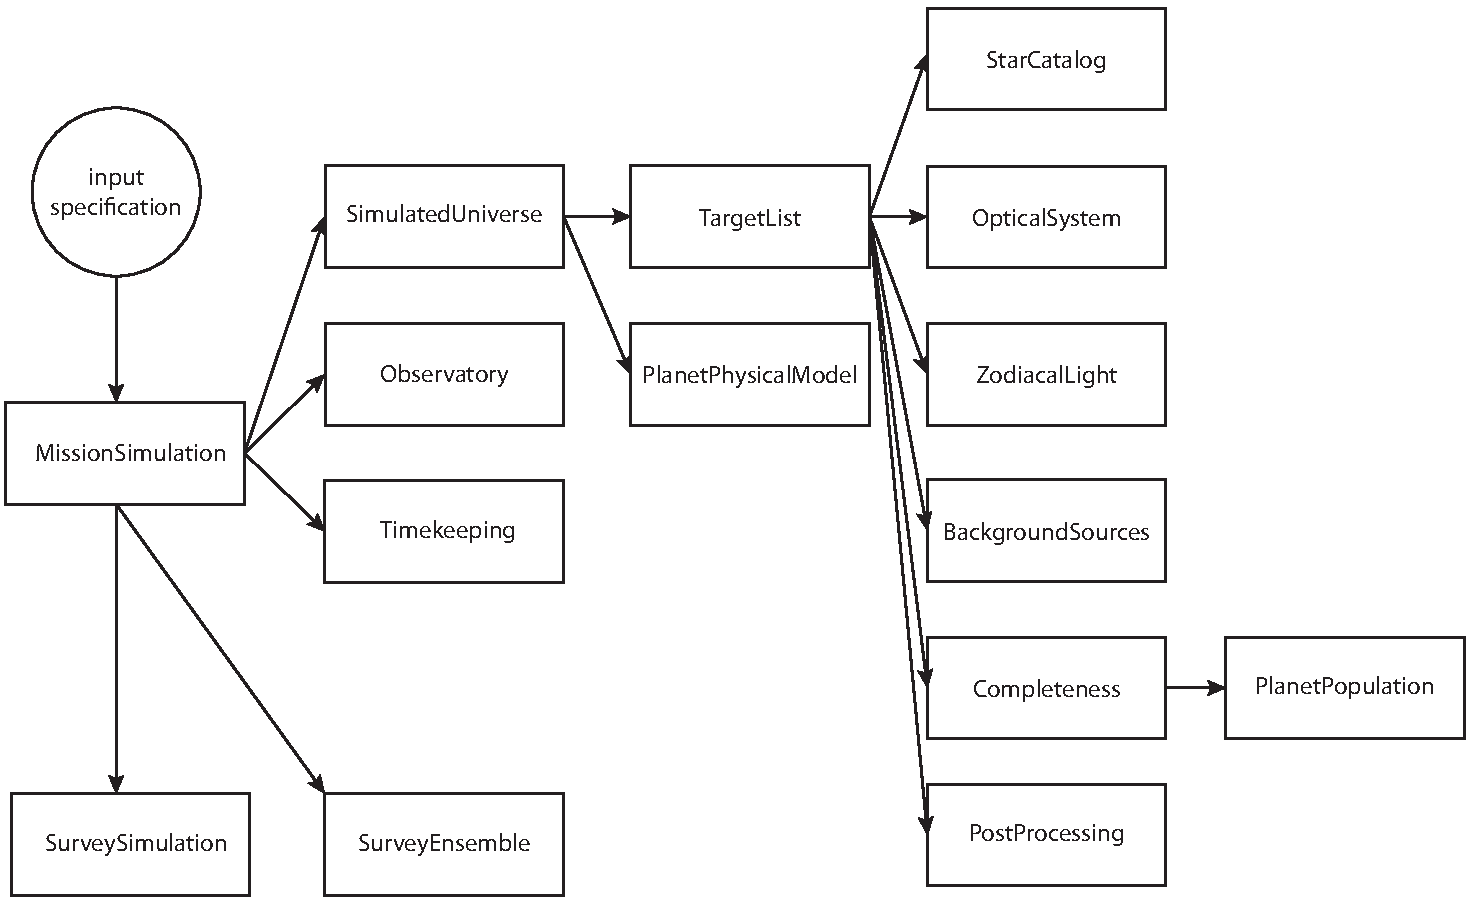
\includegraphics[width=1\textwidth]{instantiation_tree}
        \end{tabular}
    \end{center}
    \caption{Schematic depiction of the instantiation path of all simulation and input modules.  The entry point to the backbone is the construction of a MissionSimulation object, which causes the instantiation of all other module objects.  All objects are instantiated in the order shown here, with SurveySimulation and SurveyEnsemble constructed last.  The arrows indicate calls to the object constructor, and object references to each module are always passed up directly to the top calling module, so that at the end of construction, the MissionSimulation object has direct access to all other modules as its attributes.}
    \label{fig:instantiation_tree}
\end{figure}

A simulation specification is a single JSON-formatted (\url{http://json.org/}) file that encodes user-settable parameters and module names.  The backbone will contain a reference specification with \emph{all} parameters and modules set via defaults in the constructors of each of the modules.  In the initial parsing of the user-supplied specification, it will be merged with the reference specification such that any fields not set by the user will be assigned to their reference (default) values.   Each instantiated module object will contain a dictionary called \verb+_outspec+, which, taken together, will form the full specification for the current run (as defined by the loaded modules).  This specification will be written out to a json file associated with the output of every run.  \emph{Any specification added by a user implementation of any module must also be added to the \_outspec dictionary}.  The assembly of the full output specification is provided by MissionSimulation method \verb+genOutSpec+.

The backbone will also contain a specification parser that will check specification files for internal consistency.  For example, if modules carry mutual dependencies, the specification parser will return an error if these are not met for a given specification.  Similarly, if modules are selected with optional top level inputs, warnings will be generated if these are not set in the same specification files.

In addition to the specification parser, the backbone will contain a method for comparing two specification files and returning the difference between them.  Assuming that the files specify all user-settable values, this will be equivalent to simply performing a \verb+diff+ operation on any POSIX system.  The backbone diff function will add in the capability to automatically fill in unset values with their defaults.  For every simulation (or ensemble), an output specification will be written to disk along with the simulation results with all defaults used filled in.

The backbone will also contain an interactive function to help users generate specification files via a series of questions.

\subsection{Specification Format}\label{sec:inputspec}
The JSON specification file will contain a series of objects with members enumerating various user-settable parameters, top-level members for universal settings (such as the mission lifetime) and arrays of objects for multiple related specifications, such as starlight suppression systems and science instruments.  The specification file must contain a \verb+modules+ dictionary listing the module names (or paths on disk to user-implemented classes) for all modules.

\begin{verbatim}
{
  "universalParam1": value,
  "universalParam2": value,
  ...
  "starlightSuppressionSystems": [
    {
      "starlightSuppressionSystemNumber": 1,
      "type": "external",
      "detectionTimeMultiplier": value,
      "characterizationTimeMultiplier": value,
      "occulterDiameter": value,
      "NocculterDistances": 2,
      "occulterDistances: [
        {
         "occulterDistanceNumber": 1,
         "occulterDistance": value,
         "occulterBlueEdge": value,
         "occulterRedEdge": value,
         "IWA": value,
         "OWA": value,
         "PSF": "/data/mdo1_psf.fits",
         "throughput": "/data/mdo1_thru.fits",
         "contrast":  "/data1/mdo1_contrast.fits"
        },
        {
         "occulterDistanceNumber": 2,
         "occulterDistance": value,
         "occulterBlueEdge": value,
         "occulterRedEdge": value,
         "IWA": value,
         "OWA": value,
         "PSF": "/data/mdo1_psf.fits",
         "throughput": "/data/mdo1_thru.fits",
         "contrast":  "/data1/mdo1_contrast.fits"
        }
      ],
      "occulterWetMass": value,
      "occulterDryMass": value,
    },
    {
      "starlightSuppressionSystemNumber": 2,
      "type": "internal",
      "IWA": value,
      "OWA": value,
      "PSF": "/data/coron1_psf.fits",
      "throughput": "/data/coron1_thru.fits",
      "contrast":  "/data1/coron1_contrast.fits",
      "detectionTimeMultiplier": value,
      "characterizationTimeMultiplier": value,
      "opticaloh": value
    }
  ],
  "scienceInstruments": [
    {
      "scienceInstrumentNumber": 1,
      "type": "imager-EMCCD",
      "QE": 0.88,
      "darkCurrent": 9e-5,
      "CIC": 0.0013,
      "readNoise": 16,
      "texp": 1000,
      "pixelPitch": 13e-6,
      "focalLength": 240,
      "ENF": 1.414,
      "G_EM": 500
    }
    {
      "scienceInstrumentNumber": 2,
      "type": "IFS-CCD",
      "QE": 0.88,
      "darkCurrent": 9e-5,
      "CIC": 0.0013,
      "readNoise": 3,
      "texp": 1000,
      "Rspec": 70.0,
    }
  ],
  modules: {
    "PlanetPopulation": "HZEarthTwins",
    "StarCatalog": "exocat3",
    "OpticalSystem": "hybridOpticalSystem1",
    "ZodiacalLight": "10xSolZodi",
    "BackgroundSources": "besanconModel",
    "PlanetPhysicalModel": "fortneyPlanets",
    "Observatory": "WFIRSTGeo",
    "TimeKeeping": "UTCtime",
    "PostProcessing": "KLIPpost",
    "Completeness": "BrownCompleteness",
    "TargetList": "WFIRSTtargets",
    "SimulatedUniverse": "simUniverse1",
    "SurveySimulation": "backbone1",
    "SurveyEnsemble": "localIpythonEnsemble"
  }
}
\end{verbatim}

\subsection{Modules Specification}
The final array in the input specification  (\verb+modules+) is a list of all the modules that define a particular simulation.  This is the only part of the specification that will not be filled in by default if a value is missing - each module must be explicitly specified. The order of the modules in the list is arbitrary, so long as they are all present. 

If the module implementations are in the appropriate subfolder in the EXOSIMS tree, then they can be specified by the module name.  However, if you wish to use an implemented module outside of the EXOSISM directory, then you need to specify it via its full path in the input specification.

\emph{All modules, regardless of where they are stored on disk must inherit the appropriate prototype.}

\subsection{Universal Parameters}
These parameters apply to all simulations, and are described in detail in their specific module definitions:

\begin{itemize}[leftmargin=1in,font={\ttfamily}]
\item[missionLifetime] (float) The total mission lifetime in $ years $.  When the mission time is equal or greater to this value, the mission simulation stops.
\item[missionPortion] (float) The portion of the mission dedicated to exoplanet science, given as a value between 0 and 1. The mission simulation stops when the total integration time plus observation overhead time is equal to the missionLifetime $\times$ missionPortion.
\item[keepStarCatalog] (bool) Boolean representing whether to delete the star catalog after assembling the target list.  If true, object reference will be available from TargetList object.
\item[minComp] (float) Minimum completeness value for inclusion in target list. 
\item[lam] (float) Detection central wavelength in $ nm $.
\item[deltaLam] (float) Detection bandwidth in $ nm $.
\item[BW] (float) Detection bandwidth fraction = $\Delta\lambda/\lambda$.
\item[specLam] (float) Spectrograph central wavelength in $ nm $.
\item[specDeltaLam] (float) Spectrograph bandwidth in $ nm $.
\item[specBW] (float) Spectrograph bandwidth fraction = $\Delta\lambda_s/\lambda_s$.
\item[obscurFac] (float) Obscuration factor due to secondary mirror and spiders.
\item[shapeFac] (float)  Telescope aperture shape factor.
\item[pupilDiam] (float) Entrance pupil diameter in $m$.
\item[pupilArea] (float) Entrance pupil area in $m^2$.
\item[IWA] (float) Fundamental Inner Working Angle in $ arcsec $. No planets can ever be observed at smaller separations.
\item[OWA] (float) Fundamental Outer Working Angle in $ arcsec $. Set to $ Inf $ for no OWA. JSON values of 0 will be interpreted as $ Inf $.
\item[dMagLim] (float) Fundamental limiting $\Delta$mag (difference in magnitude between star and planet). 
\item[telescopeKeepout] (float) Telescope keepout angle in degrees
\item[attenuation] (float) Non-coronagraph attenuation, equal to the throughput of the optical system without the coronagraph elements.
\item[intCutoff] (float)  Maximum allowed integration time in $ days $. No integrations will be started that would take longer than this value.
\item[exozodi] (float) Mean Exo-zodi level in zodi.
\item[exozodiVar] (float) Exo-zodi variation (variance of log-normal distribution). Zodi is constant if set to zero. 
\item[FAP] (float) Detection false alarm probability
\item[MDP] (float) Missed detection probability
\item[SNimag] (float) Signal to Noise Ratio for imaging/detection.
\item[SNchar] (float) Signal to Noise Ratio for characterization.
\item[arange]   2 element list of minimum and maximum semi-major axes in $ AU $. 
\item[erange]   2 element list of minimum and maximum eccentricity.  
\item[wrange]   2 element list of minimum and maximum argument of perigee in degrees. 
\item[Orange]   2 element list of minimum and maximum ascension of the ascending node in degrees.  
\item[Irange]   2 element list of minimum and maximum inclination in degrees.  
\item[prange]   2 element list of minimum and maximum planetary geometric albedo.  
 \item[Rrange]   2 element list of minimum and maximum planetary Radius in Earth radii.  
\item[Mprange]   2 element list of minimum and maximum planetary mass in Earth masses.  
\item [scaleOrbits]   (Boolean) True means planetary orbits are scaled by the square root of stellar luminosity. 
\item[missionStart]  (float) Mission start time in $ MJD $. 
\item[missionLife]  (float) Total length of mission in $ years $. 
\item[extendedLife]  (float) Extended mission time in $ years $.  Extended life typically differs from the primary mission in some way---most typically only revisits are allowed
\item[settlingTime] (float) Amount of time needed for observatory to settle after a repointing in $ days $.             
\item[thrust] (float) Occulter slew thrust in $ mN $.
\item[slewIsp] (float) Occulter slew specific impulse in $ s $. 
\item[scMass] (float) Occulter (maneuvering spacecraft) initial wet mass in $ kg $. 
\item[dryMass] (float) Occulter (maneuvering spacecraft) dry mass in $ kg $. 
\item[coMass] (float) Telescope (or non-maneuvering spacecraft) mass in $ kg $. 
\item[skIsp] (float) Specific impulse for station keeping in $ s $. 
\item[defburnPortion] (float) Default burn portion for slewing. 
\item[spkpath] (string) Full path to SPK kernel file.
\item[forceStaticEphem]  (Boolean) Force use of static solar system ephemeris if set to True, even if jplephem module is present.
\end{itemize}

%%%%%%%%%%%%%%%%%%%%%%%%%%%%%%%%%%%%%%%%%%%%%%%%%%%%%%%%%%%%%%%%%%%%%%%%%
% INPUT MODULES DESCRIPTION
%%%%%%%%%%%%%%%%%%%%%%%%%%%%%%%%%%%%%%%%%%%%%%%%%%%%%%%%%%%%%%%%%%%%%%%%%

\section{Input Modules}\label{sec:modules}
The input modules include Planet Population, Star Catalog, Optical System, Zodiacal Light, Background Sources, Planet Physical Model, Observatory, Time Keeping, and Post-Processing.  These modules encode and/or generate all of the information necessary to perform mission simulations.  The specific mission design determines the functionality of each input module, while inputs and outputs of these modules remain the same (in terms of data type and variable representations).  This section defines the functionality, major tasks, input, output, and interface of each of these modules.

% PLANET POPULATION

\subsection{Planet Population}
The Planet Population module encodes the density functions of all required planetary parameters, both physical and orbital. These include semi-major axis, eccentricity, orbital orientation, radius, mass, and geometric albedo (see \S\ref{sec:pdfs}). Certain parameter models may be empirically derived while others may come from analyses of observational surveys.  This module also encodes the limits on all parameters to be used for sampling the distributions and determining derived cutoff values such as the maximum target distance for a given instrument's IWA.

\begin{figure}[ht]
    \begin{center}
        \begin{tabular}{c}
             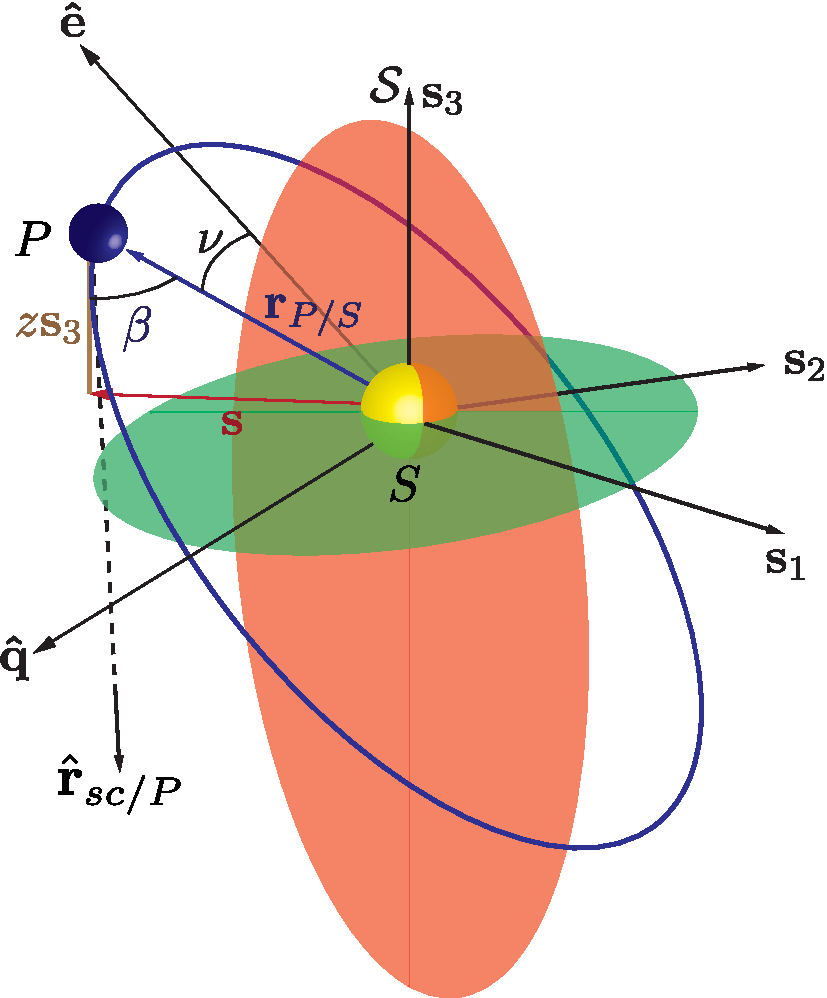
\includegraphics[width=0.6\textwidth]{orbit_diagram}
        \end{tabular}
    \end{center}
    \caption{\label{fig:orbit_diagram} Definition of reference frames and coordinates of simulated exosystems.  The observer lies along the negative $\mf s_3$ axis so that the observer-star unit vector is $+\mf s_3$.}
\end{figure}

The coordinate system of the simulated exosystems is defined as in \reffig{fig:orbit_diagram}.  The observer looks at the target star along the $\mathbf{s}_3$ axis, located at a distance $-d\mathbf{s}$ from the target at the time of observation. The argument of periapse, inclination,  and longitude of the ascending node ($\omega, I, \Omega$) are defined as a 3-1-3 rotation about the unit vectors defining the $\mathcal{S}$ reference frame.  This rotation defines the standard Equinoctial reference frame ($\mfhat{e}, \mfhat{q}, \mfhat{h}$), with the true anomaly ($\nu$) measured from $\mfhat{e}$).  The planet-star orbital radius vector $\mf r_{P/S}$ is projected into the $\mf s_1, \mf s_2$ plane as the projected separation vector $\mf s$, with magnitude $s$, and the phase (star-planet-observer) angle ($\beta$) is closely approximated by the angle between $\mf r_{P/s}$ and its projection onto $\mf s_3$.

The Planet Population module does not model the physics of planetary orbits or the amount of light reflected or emitted by a given planet, but rather encodes the statistics of planetary occurrence and properties. 

\label{sec:planetpopulation}
\subsubsection{Planet Population Object Attribute Initialization Input/Output Description} 
\subsubsection*{Inputs}
The following are all entries in the passed specs dictionary (derived from the JSON script file or another dictionary).  Values not specified will be replaced with defaults, as listed.  It is important to note that many of these (in particular mass and radius) may be mutually dependent, and so some implementation may choose to only use some for inputs and set the rest via the physical models.

\begin{itemize}
\item
\begin{description}
    \item[arange] \hfill \\
    2 element list of minimum and maximum semi-major axes in $ AU $. Default value is [0.01, 100]
    \item[erange] \hfill \\
    2 element list of minimum and maximum eccentricity.  Default value is [0.01,0.99]
    \item[wrange] \hfill \\
    2 element list of minimum and maximum argument of perigee in degrees.  Default value is [0,360]
    \item[Orange] \hfill \\
    2 element list of minimum and maximum ascension of the ascending node in degrees.  Default value is [0,360]
    \item[Irange] \hfill \\
    2 element list of minimum and maximum inclination in degrees.  Default value is [0,180]
    \item[prange] \hfill \\
    2 element list of minimum and maximum planetary geometric albedo.  Default value is [0.1,0.6]
     \item[Rrange] \hfill \\
    2 element list of minimum and maximum planetary Radius in Earth radii.  Default value is [1, 30]
    \item[Mprange] \hfill \\
    2 element list of minimum and maximum planetary mass in Earth masses.  Default value is [1, 4131]
\end{description}
\end{itemize}

\subsubsection*{Attributes}
\begin{itemize}
    \item
    \begin{description}
        \item[arange] \hfill \\
        Semi-major axis range defined as [a\_min, a\_max] (astropy Quantity initially set in $ AU $)
        \item[erange] \hfill \\
        Eccentricity range defined as [e\_min, e\_max]
        \item[wrange] \hfill \\
        Argument of perigee range defined as [w\_min, w\_max] (astropy Quantity initially set in degrees)
        \item[Orange] \hfill \\
        Right ascension of the ascending node range defined as [O\_min, O\_max]  (astropy Quantity initially set in degrees)
        \item[prange] \hfill \\
        Planetary geometric albedo range defined as [p\_min, p\_max]
        \item[Irange] \hfill \\
        Planetary orbital inclination range defined as [I\_min, I\_max]  (astropy Quantity initially set in degrees)
        \item[Rrange] \hfill \\
        Planetary radius range defined as [R\_min, R\_max] (astropy Quantity initially set in $ m $)
        \item[Mprange] \hfill \\
        Planetary mass range defined as [Mp\_min, Mp\_max] (astropy Quantity initially set in $ kg $)
        \item[rrange] \hfill \\
        Planetary orbital radius range defined as [r\_min, r\_max] derived from PlanetPopulation.arange and PlanetPopulation.erange (astropy Quantity initially set in $ AU $)
     \item [scaleOrbits] \hfill \\
    Boolean where True means planetary orbits are scaled by the square root of stellar luminosity. Default value is False.
         \item[PlanetPhysicalModel] \hfill \\     
            Planet physical model object
    \end{description}
\end{itemize}

\subsubsection{Planet Population Value Generators} \label{sec:pdfs}
For each of the parameters represented by the input attributes, the planet population object will provide a method that returns random values for the attribute, within the ranges specified by the attribute (so that, for example, there will be a \verb+gen_sma+ method corresponding to \verb+arange+, etc.).  Each of these methods will take a single input of the number of values to generate.  These methods will encode the probability density functions representing each parameter, and use either a rejection sampler or other (numpy or scipy) provided sampling method to generate random values.  All returned values will have the same type/default units as the attributes. 

In cases where values need to be sampled jointly (for example if you have a joint distribution of semi-major axis and planetary radius) then the sampling will be done by a helper function which stores the last sampled values in memory, and the individual functions (i.e., \verb+gen_sma+ and \verb+gen_radius+) will act as getters for the values.  In cases where there is a deterministic calculation of one parameter from another (as in mass calculated from radius) this will be provided separately in the Planet Physical module. Any non-standard distribution functions being sampled by one of these methods should be created as object attributes in the implementation constructor so that they are available to other modules.
\\\\
The methods are:

\begin{itemize}
    \item 
    \begin{description}
        \item[gen\_sma] \hfill \\
        Returns semi-major axis values (astropy Quantity initially set in $ AU $)
        \item[gen\_eccentricity] \hfill \\
        Returns eccentricity values (numpy ndarray)
        \item[gen\_w] \hfill \\
        Returns argument of perigee values (astropy Quantity initially set in degrees)
        \item[gen\_O] \hfill \\
        Returns longitude of the ascending node values (astropy Quantity initially set in degrees)
        \item[gen\_radius] \hfill \\
        Returns planetary radius values  (astropy Quantity initially set in $ m $)
        \item[gen\_mass] \hfill \\
        Returns planetary mass values (astropy Quantity initially set in $ kg $)
        \item[gen\_albedo] \hfill \\
        Returns planetary geometric albedo (numpy ndarray)
        \item[gen\_I] \hfill \\
        Returns values of orbital inclination (astropy Quantity initially set in degrees)
    \end{description}
\end{itemize}

% PLANET PHYSICAL MODEL 

\subsection{Planet Physical Model} \label{sec:planetphysicalmodel}
The Planet Physical Model module contains models of the light emitted or reflected by planets in the wavelength bands under investigation by the current mission simulation.  It takes as inputs the physical quantities sampled from the distributions in the Planet Population module and generates synthetic spectra (or band photometry, as appropriate).  The specific implementation of this module can vary greatly, and can be based on any of the many available planetary geometric albedo, spectra and phase curve models.  As required, this module also provides physical models relating dependent parameters that cannot be sampled independently (for example density models relating plant mass and radius).  While the specific methods will depend highly on the physical models being used, the prototype provides three stubs that will be commonly useful:

\begin{itemize}
    \item 
    \begin{description}
        \item[calc\_albedo\_from\_sma] \hfill \\
        Provides a method to calculate planetary geometric albedo as a function of the semi-major axis
        \item[calc\_mass\_from\_radius] \hfill \\
        Provides a method to calculate planetary masses from their radii
        \item[calc\_radius\_from\_mass] \hfill \\
        Provides a method to calculate planetary radii from their masses
    \end{description}
\end{itemize}



% STAR CATALOG

\subsection{Star Catalog} \label{sec:starcatalog}
The Star Catalog module includes detailed information about potential target stars drawn from general databases such as SIMBAD, mission catalogs such as Hipparcos, or from existing curated lists specifically designed for exoplanet imaging missions.  Information to be stored, or accessed by this module will include target positions and proper motions at the reference epoch, catalog identifiers (for later cross-referencing), bolometric luminosities, stellar masses, and magnitudes in standard observing bands.  Where direct measurements of any value are not available, values are synthesized from ancillary data and empirical relationships, such as color relationships and mass-luminosity relations.

This module does not provide any functionality for picking the specific targets to be observed in any one simulation, nor even for culling targets from the input lists where no observations of a planet could take place.  This is done in the Target List module as it requires interactions with the Planet Population (to determine the population of interest), Optical System (to define the capabilities of the instrument), and Observatory (to determine if the view of the target is unobstructed) modules.

\subsubsection{Star Catalog Object Attribute Initialization Input/Output Description} 
The Star Catalog prototype creates empty 1D NumPy ndarrays for each of the output quantities listed below.  Specific Star Catalog modules must populate the values as appropriate.  Note that values that are left unpopulated by the implementation will still get all zero array, which may lead to unexpected behavior.

\subsubsection*{Inputs}
\begin{itemize}
    \item 
    \begin{description}
        \item[star catalog information] \hfill \\
        Information from an external star catalog (left deliberately vague as these can be anything).
    \end{description}
\end{itemize}

\subsubsection*{Attributes}
\begin{itemize}
    \item 
    \begin{description}
        \item[StarCatalog.Name] \hfill \\
        1D NumPy ndarray of star names
        \item[StarCatalog.Type] \hfill \\
        1D NumPy ndarray of star types
        \item[StarCatalog.Spec] \hfill \\
        1D NumPy ndarray of spectral types
        \item[StarCatalog.parx] \hfill \\
        1D NumPy ndarray of parallax in $ mas $
        \item[StarCatalog.Umag] \hfill \\
        1D NumPy ndarray of U magnitude
        \item[StarCatalog.Bmag] \hfill \\
        1D NumPy ndarray of B magnitude
        \item[StarCatalog.Vmag] \hfill \\
        1D NumPy ndarray of V magnitude
        \item[StarCatalog.Rmag] \hfill \\
        1D NumPy ndarray of R magnitude
        \item[StarCatalog.Imag] \hfill \\
        1D NumPy ndarray of I magnitude
        \item[StarCatalog.Jmag] \hfill \\
        1D NumPy ndarray of J magnitude
        \item[StarCatalog.Hmag] \hfill \\
        1D NumPy ndarray of H magnitude
        \item[StarCatalog.Kmag] \hfill \\
        1D NumPy ndarray of K magnitude
        \item[StarCatalog.dist] \hfill \\
        1D NumPy ndarray of distance in parsecs
        \item[StarCatalog.BV] \hfill \\
        1D NumPy ndarray of B-V Johnson magnitude
        \item[StarCatalog.MV] \hfill \\
        1D NumPy ndarray of absolute V magnitude
        \item[StarCatalog.BC] \hfill \\
        1D NumPy ndarray of bolometric correction
        \item[StarCatalog.L] \hfill \\
        1D NumPy ndarray of stellar luminosity in Solar luminosities
        \item[StarCatalog.coords] \hfill \\
        Astropy \href{http://astropy.readthedocs.org/en/latest/api/astropy.coordinates.SkyCoord.html}{SkyCoord object} containing list of star positions (e.g., right ascension and declination)
        \item[StarCatalog.pmra] \hfill \\
        1D NumPy ndarray of proper motion in right ascension in $ mas/year $
        \item[StarCatalog.pmdec] \hfill \\
        1D NumPy ndarray of proper motion in declination in $ mas/year $
        \item[StarCatalog.rv] \hfill \\
        1D NumPy ndarray of radial velocity in kilometers/second
        \item[StarCatalog.Binary\_Cut] \hfill \\
        Boolean 1D NumPy ndarray where True is companion star closer than $ 10 arcsec $
    \end{description}
\end{itemize}

\subsection{Optical System}
The Optical System module contains all of the necessary information to describe the effects of the telescope and starlight suppression system on the target star and planet wavefronts.  This requires encoding the design of both the telescope optics and the specific starlight suppression system, whether it be an internal coronagraph or an external occulter.  The encoding can be achieved by specifying Point Spread Functions (PSF) for on- and off-axis sources, along with angular separation and wavelength dependent contrast and throughput definitions.  At the opposite level of complexity, the encoded portions of this module may be a description of all of the optical elements between the telescope aperture and the imaging detector, along with a method of propagating an input wavefront to the final image plane.  Intermediate implementations can include partial propagations, or collections of static PSFs representing the contributions of various system elements.  The encoding of the optical train will allow for the extraction of specific bulk parameters including the instrument inner working angle (IWA), outer working angle (OWA), and mean and max contrast and throughput.

Finally, the Optical System must also include a description of the science instrument.  The baseline instrument is assumed to be an imaging spectrometer.  The encoding must provide the spatial and wavelength coverage of the instrument as well as sampling for each, along with detector details such as read noise, dark current, and readout cycle.

The Optical System module has two methods used in simulation.  \verb+calc_maxintTime+ is called from the Target List module to calculate the maximum integration time for each star in the target list (see \S\ref{sec:calcmaxintTimetask}).  \verb+calc_intTime+ is called from the Survey Simulation module to calculate integration times for a target system (see \S\ref{sec:calcintTimetask}).  The inputs and outputs for the Optical System methods are depicted in \reffig{fig:opticalsysmodule}.

\begin{figure}[ht]
    \begin{center}
        \begin{tabular}{c}
             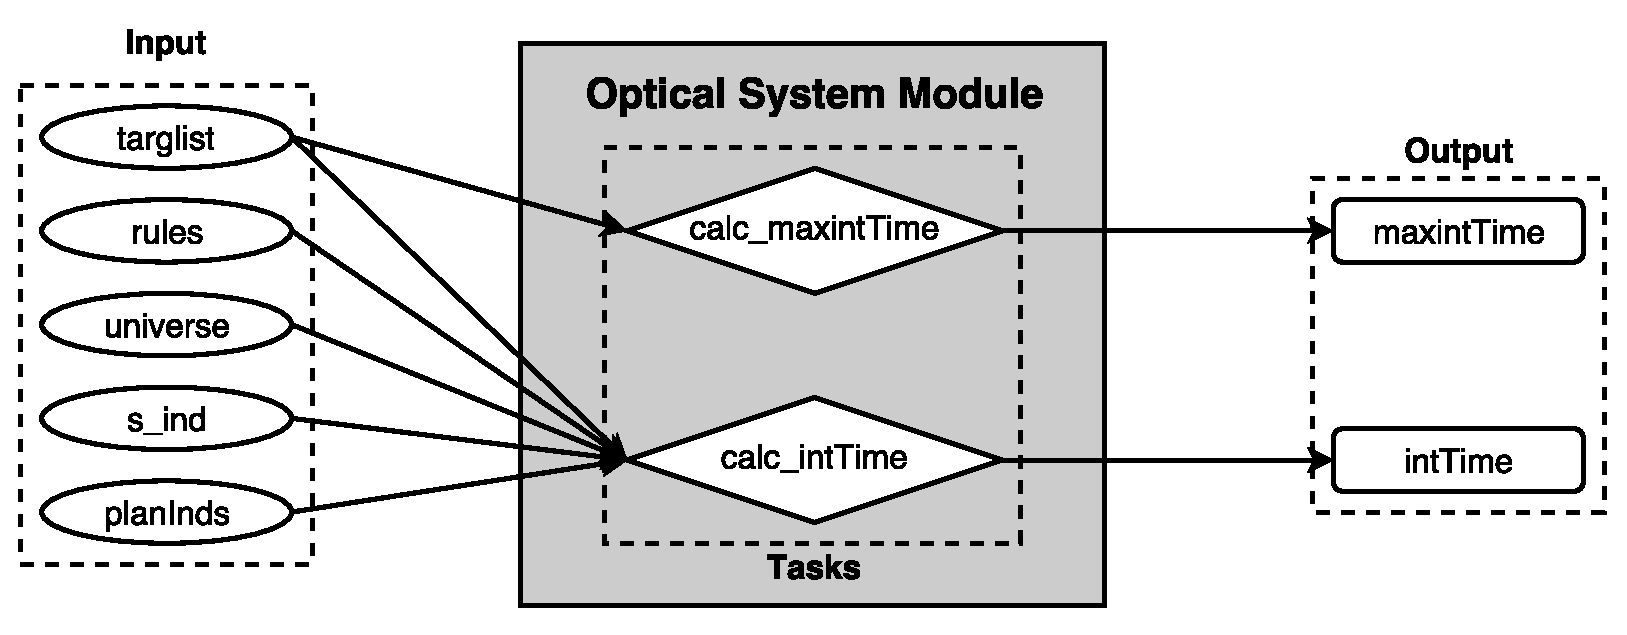
\includegraphics[width=\textwidth]{OpticalSysTasks}
        \end{tabular}
    \end{center}
    \caption{\label{fig:opticalsysmodule} Depiction of Optical System module methods including inputs and outputs (see \S\ref{sec:calcmaxintTimetask} and \S\ref{sec:calcintTimetask}).}
\end{figure}


\label{sec:opticalsystem}
\subsubsection{Optical System Object Attribute Initialization Input/Output Description} 

The specific set of inputs to this module will vary based on the simulation approach used.  Here we define the specification for the case where static PSF(s), derived from external diffraction modeling, are used to describe the system.  Note that some of the inputs are coronagraph or occulter specific, and will be expected based on the "internal" or "external" starlight suppression system keyword, respectively.


\subsubsection*{Inputs}
Information from simulation specification JSON file organized into a Python dictionary.  For multiple systems, there will be an array of dictionaries. If the below key: value pairs are missing from the input specification, the Optical System object attributes will be assigned the default values listed. The following are all entries in the passed specs dictionary.

\begin{itemize}
    \item 
\begin{description}
    \item[lam] \hfill \\
    Detection central wavelength in $ nm $. Default value is 500.
    \item[deltaLam] \hfill \\
    Detection bandwidth $ \Delta\lambda $ in $ nm $.
    \item[BW] \hfill \\ Detection bandwidth fraction $(\Delta\lambda/\lambda)$. Only applies when deltaLam is not specified. Default value is 0.2.
    \item[specLam] \hfill \\
    Spectrograph central wavelength in $ nm $. Default value is equal to lam.
    \item[specDeltaLam] \hfill \\
    Spectrograph bandwidth $\Delta\lambda_s$ in $ nm $.
    \item[specBW] \hfill \\
    Spectrograph bandwidth fraction $(\Delta\lambda_s/\lambda_s)$. Only applies when specDeltaLam is not specified. Default value is BW.
    \item[obscurFac] \hfill \\
    Obscuration factor due to secondary mirror and spiders. Default value is 0.2.
    \item[shapeFac] \hfill \\
    Shape factor (also known as fill factor) so that $ shapeFac \times diameter^2 = Area $. Default value is $ \frac{\pi}{4} $.
    \item[pupilDiam] \hfill \\
    Entrance pupil diameter in  $ m $. Default value is $ 4$.
    \item[IWA] \hfill \\
    Fundamental Inner Working Angle in $ arcsec $. No planets can ever be observed at smaller separations. If not set, defaults to smallest IWA of all starlightSuppressionSystems.
    \item[OWA] \hfill \\
    Fundamental Outer Working Angle in $ arcsec $. Set to $ Inf $ for no OWA. If not set, defaults to largest OWA of all starlightSuppressionSystems.  JSON values of 0 will be interpreted as $ Inf $.
    \item[dMagLim] \hfill \\
    Fundamental limiting $ \Delta$mag (difference in magnitude between star and planet). Default value is minimum of contrast.
    \item[telescopeKeepout] \hfill \\
    Telescope keepout angle in degrees
    \item[attenuation] \hfill \\
    Non-coronagraph attenuation, equal to the throughput of the optical system without the coronagraph elements. Default value is 0.57.
    \item[intCutoff] \hfill \\
    Maximum allowed integration time in $ days $. Default value is 50. No integrations will be started that would take longer than this value.
    \item[Npix] \hfill \\
    Number of noise pixels. Default value is 14.3.
    \item[Ndark] \hfill \\
    Number of dark frames used. Default value is 10.

    \item[starLightSuppressionSystems] \hfill\\ Array of dictionaries containing these (or other) starlight suppression system values.
    \begin{description}
    \item[starlightSuppressionSystemNumber] \hfill\\ (Required) Integer counter of the system.
    \item[type] \hfill\\ (Required) String indicating type of sytems.  Standard values are `internal',`external', and `hybrid'.
    \item[IWA] \hfill \\
     Inner Working Angle of this system in $ arcsec $. If not set, or if too small for this system contrast/throughput definitions, defaults to smallest WA of contrast/throughput definitions.
    \item[OWA] \hfill \\
    Specific Outer Working Angle of this system in $ arcsec $. Set to $ Inf $ for no OWA. If not set, or if too large for this system contrast/throughput definitions, defaults to largest WA of contrast/throughput definitions.  JSON values of 0 will be interpreted as $ Inf $.
    \item[dMagLim] \hfill \\
    Limiting $ \Delta$mag for this system. Default value is minimum of the system contrast.
    \item[throughput] \hfill \\
    Coronagraph throughput: either a scalar for constant throughput, a two-column array for angular separation-dependent throughput, where the first column contains the separations in $ arcsec $, or a 2D array for angular separation- and wavelength- dependent throughput, where the first column contains the angular separation values in as and the first row contains the wavelengths in $ nm $.  The ranges on all parameters must be consistent with the values for the IWA, OWA, lam and deltaLam inputs.  May be data or FITS filename. Default is scalar 0.5.
    \item[contrast] \hfill \\
    Optical system contrast: either a scalar for constant contrast, a two-column array for angular separation-dependent contrast, where the first column contains the separations in $ arcsec $, or a 2D array for angular separation- and wavelength- dependent contrast, where the first column contains the angular separation values in as and the first row contains the wavelengths in $ nm $.  The ranges on all parameters must be consistent with the values for the IWA, OWA, lam and deltaLam inputs. May be data or FITS filename. Default is scalar 1e-10.
    \item[PSF] \hfill \\
    Instrument point spread function. Either a 2D array of a single-PSF, or a 3D array of wavelength-dependent PSFs. May be data or FITS filename. Default is numpy.ones((3,3)).
    \item[PSFsampling] \hfill \\
    Sampling of the PSF in $ arcsec/pixel $. Default value is 10.
    \item[detectionTimeMultiplier]\hfill \\
    Duty cycle of a detection observation.  If only a single integration is required for the initial detection observation, then this value is 1.  Otherwise, it is equal to the number of discrete integrations needed to cover the full field of view (i.e., if a shaped pupil with a dark hole that covers 1/3 of the field of view is used for detection, this value would equal 3).  Defaults to 1.
    \item[characterizationTimeMultiplier]\hfill \\
    Characterization duty cycle.  If only a single integration is required for the initial detection observation, then this value is 1.  Otherwise, it is equal to the number of discrete integrations needed to cover the full wavelength band and all required polarization states.  For example, if the band is split into three sub-bands, and there are two polarization states that must be measured, and each of these must be done sequentially, then this value would equal 6.  However, if the three sub-bands could be observed at the same time (e.g., by separate detectors) then the value would by two (for the two polarization states). Defaults to 1.
    \item[opticaloh] \hfill \\
    Optical system overhead time in $ days $.  Default value is 1 day.  This is the (assumed constant) amount of time required to set up the optical system (i.e., dig the dark hole or do fine alignment with the occulter).  It is added to every observation, and is separate from the observatory overhead defined in the observatory module, which represents the observatory's settling time.  Both overheads are added to the integration time to determine the full duration of each detection observation.
    \item[occulterDiameter]\hfill \\
    Occulter diameter in $ m $.  Measured petal tip-to-tip.
    \item [NocculterDistances]\hfill \\
    Number of telescope separations the occulter operates over (number of occulter bands). If greater than 1, then the occulter description is an array of dicts.
    \item[occulterDistance]\hfill \\
    Telescope-occulter separation in $km$.
    \item[occulterBlueEdge]\hfill \\
    Occulter blue end of wavelength band in $nm$.
    \item[occulterRedEdge]\hfill \\
    Occulter red end of wavelength band in $nm$.
    \end{description}
    
    \item[scienceInstruments] \hfill\\ Array of dictionaries containing these (or other) detector system values.  Defaults are filled in only when listed.
    \begin{description}
    \item[scienceInstrumentNumber] \hfill\\ (Required) Integer counter of the system.
    \item[type] \hfill\\ (Required) String indicating type of system.  Standard values are `imaging' and `spectro'.
    \item[darkCurrent] \hfill \\
    Detector dark-current rate in units of $ electrons /s /pix $ (float). 
    \item[readNoise] \hfill \\
    Detector read noise in $ electrons/frame $ (float). 
    \item[texp] \hfill \\
    Exposure time in $ s/frame $. 
    \item[QE] \hfill \\
    Detector quantum efficiency: either a scalar for constant QE, or a two-column array for wavelength-dependent QE, where the first column contains the wavelengths in $ nm $. The ranges on all parameters must be consistent with the values for lam and deltaLam inputs. May be data or FITS filename. 
    \item[pixelPitch] \hfill \\
    Pixel pitch in $ m $ (float). 
    \item[focalLength] \hfill \\
    Focal length in $ m $ (float). 
    \item[Rspec] \hfill \\
    (Specific to spectrometers) Spectral resolving power defined as $\lambda/d\lambda$ (float). 
    \item[CIC] \hfill \\
    (Specific to CCDs) Clock-induced-charge in units of $ electrons/pix/frame $
    \item[ENF] \hfill \\
    (Specific to EM-CCDs) Excess noise factor (float).
    \item[G\_EM] \hfill \\
    (Specific to EM-CCDs) Electron multiplication gain    \end{description}
\end{description}
\end{itemize}
For all values that may be either scalars or interpolants, in the case where scalar values are given, the optical system module will automatically wrap them in lambda functions so that they become callable (just like the interpolant) but will always return the same value for all arguments.  The inputs for interpolants may be filenames (full absolute paths) with tabulated data, or NumPy ndarrays of argument and data (in that order in rows so that input[0] is the argument and input[1] is the data).  When the input is derived from a JSON file, these must either be scalars or filenames.

The starlight suppression system and science instrument dictionaries can contain any other attributes required by a particular optical system implementation.  The only significance of the ones enumerated above is that they are explicitly checked for by the prototype constructor, and cast to their expected values.

In cases where there is only one starlight suppression system and/or one science instrument, all values from those dictionaries are copied directly to the OpticalSystem object and can be accessed as direct attributes (i.e., \verb+OpticalSystem.Rspec+, etc.).

\subsubsection*{Attributes}
These will always be present in an OpticalSystem object and directly accessible as \verb+OpticalSystem.Attribute+.
\begin{itemize}
\item 
\begin{description}
    \item[lam] \hfill \\
    Detection wavelength (astropy Quantity initially set in $ nm $)
    \item[deltaLam] \hfill \\
    Detection bandwidth $ \Delta\lambda $ (astropy Quantity initially set in $ nm $)
    \item[obscurFac] \hfill \\
    Obscuration factor due to secondary mirror and spiders
    \item[shapeFac] \hfill \\
    Shape factor of the unobscured pupil area, so that $ shapeFac \times pupilDiam^2  \times (1-obscurFac) = pupilArea $
    \item[pupilDiam] \hfill \\
    Entrance pupil diameter (astropy Quantity initially set in $ m $)
    \item[pupilArea] \hfill \\
    Entrance pupil area (astropy Quantity initially set in $ m^{2} $)
    \item[SNchar] \hfill \\
    Signal to Noise Ratio for characterization
    Focal length (astropy Quantity initially set in $ m $)
    \item[IWA] \hfill \\
    Fundamental Inner Working Angle (astropy Quantity initially set in $ arcsec $)
    \item[OWA] \hfill \\
    Fundamental Outer Working Angle (astropy Quantity initially set in $ as $)
    \item[dMagLim] \hfill \\
    Fundamental Limiting $ \Delta$mag (difference in magnitude between star and planet)
    \item[telescopeKeepout] \hfill \\
    Telescope keepout angle (astropy Quantity initially set in degrees)
    \item[attenuation] \hfill \\
    Non-coronagraph attenuation, equal to the throughput of the optical system without the coronagraph elements (float).
    \item[specLam] \hfill \\
    Spectral wavelength of interest (astropy Quantity initially set in $ nm $)
    \item[intCutoff] \hfill \\
    Maximum allowed integration time (astropy Quantity initially set in $ days $)
    \item[starlightSuppressionSystems] \hfill \\  Array of dicts containing all supplied starlight suppression system attributes.  Only required attributes are `starlightSuppressionSystemNumber' and `type'.  Typically the first system will be the one used for imaging, and the second one for spectroscopy, but this is not a requirement.  See above for other commonly used attributes.
    \item[scienceInstruments] \hfill \\  Array of dicts containing all supplied science instrument attributes.  Only required attributes are `scienceInstrumentNumber' and `type'.  Typically the first system will be the one used for imaging, and the second one for spectroscopy, but this is not a requirement.  See above for other commonly used attributes.
\end{description}
\end{itemize}
In cases where either of the two attribute dictionary lists (starlight suppression systems and science instruments) only contain one dictionary (i.e., there's only one coronagraph and/or detector), then all attributes will be linked as direct attributes of the object as well as stored in the dictionary.

\subsubsection{calc\_maxintTime Method Input/Output Description} \label{sec:calcmaxintTimetask}
The \verb+calc_maxintTime+ method calculates the maximum integration time for each star in the target list.  This method is called from the Target List module.
\subsubsection*{Inputs}
\begin{itemize}
    \item 
    \begin{description}
        \item[targlist] \hfill \\
        Instantiated TargetList object from TargetList module see \S\ref{sec:targetlist} for definition of available attributes
    \end{description}
\end{itemize}

\subsubsection*{Output}
\begin{itemize}
    \item
    \begin{description}
        \item[maxintTime] \hfill \\
        Maximum integration time for each target star as 1D NumPy ndarray with astropy Quantity units of time attached
    \end{description}
\end{itemize}

\subsubsection{calc\_intTime Method Input/Output Description} \label{sec:calcintTimetask}
The \verb+calc_intTime+ method calculates the integration time required for a specific target system.  This method is called from the Survey Simulation module.
\subsubsection*{Inputs}
\begin{itemize}
    \item 
    \begin{description}
        \item[targlist] \hfill \\
        Instantiated TargetList object from TargetList module see \S\ref{sec:targetlist} for definition of available attributes
        \item[starInd] \hfill \\
        Numpy ndarray containing integer indices of the stars of interest, with the length of the number of planets of interest. For instance, if a star hosts $n$ planets, the index of this star must be repeated $n$ times.
        \item[dMagPlan] \hfill \\
        Numpy ndarray containing differences in magnitude between planets and their host star, with the length of the number of planets of interest.
        \item[WA] \hfill \\
        Numpy ndarray containing working angles of the planets of interest
        \item[I] \hfill \\
        Numpy ndarray containing inclinations of the planets of interest
    \end{description}
\end{itemize}

\subsubsection*{Output}
\begin{itemize}
    \item 
    \begin{description}
        \item[intTime] \hfill \\
        Integration time for each of the planets of interest as 1D NumPy ndarray with astropy Quantity units of time in $ days $
    \end{description}
\end{itemize}

% ZODIACAL LIGHT 

\subsection{Zodiacal Light}\label{sec:zodiacallight}

The Zodiacal Light module contains the \verb+fzodi+ method.  This method calculates the contribution of both local and exozodiacal light levels for each planet.  The inputs and outputs for the Zodiacal Light method are depicted in \reffig{fig:zodiacallightmodule}.

\begin{figure}[ht]
    \begin{center}
        \begin{tabular}{c}
             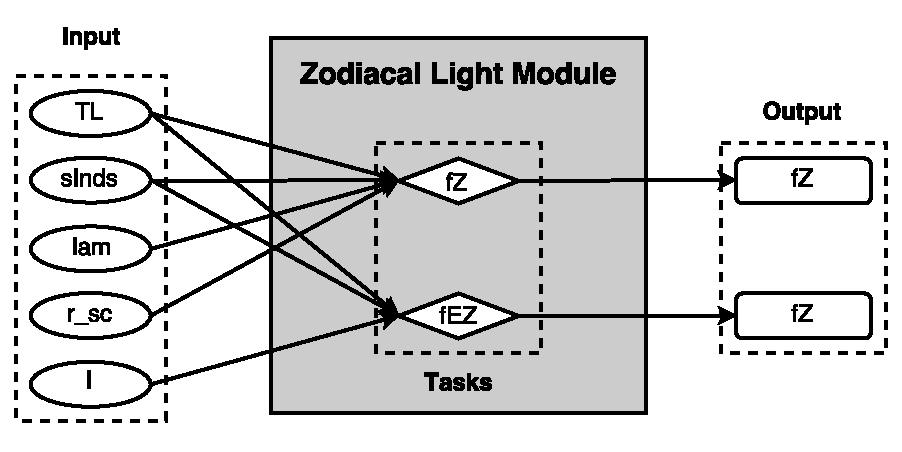
\includegraphics[width=0.8\textwidth]{ZodiTasks}
        \end{tabular}
    \end{center}
    \caption{\label{fig:zodiacallightmodule} Depiction of Zodiacal Light module method including inputs and outputs (see \S\ref{sec:fzoditask}).}
\end{figure}

\subsubsection{Zodiacal Light Object Attribute Initialization Input/Output Description}
\subsubsection*{Input}
\begin{itemize}
\item
\begin{description}
    \item
            \item[exozodi] \hfill \\
            Exo-zodi level in zodi. Defaults to 1.5.
            \item[exozodiVar] \hfill \\
            Exo-zodi variation (variance of log-normal distribution). Zodi is constant if set to zero.  Defaults to 0.
            \item[exozodiMag] \hfill \\
            1 exo-zodi brightness in $ mag/asec^2 $. Defaults to 23.54.
\end{description}
\end{itemize}

\subsubsection*{Attributes}
\begin{itemize}
\item
\begin{description}
        \item[exozodi] \hfill \\
        Exo-zodi level in zodi
        \item[exozodiVar] \hfill \\
        Exo-zodi variation (variance of log-normal distribution). Zodi is constant if set to zero.
        \item[exozodiMag] \hfill \\
        1 exo-zodi brightness in $ mag/asec^2 $.
\end{description}
\end{itemize}

\subsubsection{fzodi Method Input/Output Description} \label{sec:fzoditask}
The \verb+fzodi+ method returns exozodi levels for planetary systems.  This functionality is used by the Simulated Universe module.

\subsubsection*{Inputs}
\begin{itemize}
    \item 
    \begin{description}
        \item[Inds] \hfill \\
        1D NumPy ndarray of indices mapping planets to stars contained in the target list
        \item[I] \hfill \\
        1D NumPy ndarray of planet inclination in degrees
        \item[targlist] \hfill \\
        Instantiated Target List object from Target List module see \S\ref{sec:targetlist} for description of functionality and attributes
    \end{description}
\end{itemize}

\subsubsection*{Outputs}
\begin{itemize}
    \item 
    \begin{description}
        \item[fzodicurr] \hfill \\
        1D NumPy ndarray containing exozodiacal light levels in zodi
    \end{description}
\end{itemize}

\subsection{Background Sources}\label{sec:backgroundsources}

The Background Sources module will provide density of background sources for a given target based on its coordinates and the integration depth.  This will be used in the post-processing module to determine false alarms based on confusion.  The prototype module has no inputs and only a single function: \verb+dNbackground+.

\subsubsection{dNbackground}
\subsubsection*{Inputs}
\begin{itemize}
    \item 
    \begin{description}
        \item[coords] \hfill \\
        Astropy \href{http://astropy.readthedocs.org/en/latest/api/astropy.coordinates.SkyCoord.html}{SkyCoord object} containing list of star positions (e.g., right ascension and declination), typically passed from target list.
        \item[intDepths] \hfill \\
        Array-like (list or ndarray) of floating point values equal to absolute magnitude (in the detection band) of dark hole to be produced for each target. Dimension must match the length of the coords input.
    \end{description}
\end{itemize}

\subsubsection*{Outputs}
\begin{itemize}
    \item 
    \begin{description}
        \item[dN] \hfill \\
        Numpy ndarray matching size of inputs, containing number densities of background sources for given targets in number per square arcminute.
    \end{description}
\end{itemize}


% OBSERVATORY

\subsection{Observatory}
The Observatory module contains all of the information specific to the space-based observatory not included in the Optical System module. The module has two main methods: \verb+orbit+ and \verb+keepout+, which are implemented as functions within the module. 

The observatory orbit plays a key role in determining which of the target stars may be observed for planet finding at a specific time during the mission lifetime. The Observatory module's \verb+orbit+ method takes the current mission time as input and outputs the observatory's position vector. The position vector is standardized throughout the modules to be referenced to a heliocentric equatorial frame at the J2000 epoch. The observatory's position vector is used in the \verb+keepout+ method and Target List module to determine which of the stars are observable at the current mission time.

The \verb+keepout+ method determines which target stars are observable at a specific time during the mission simulation and which are unobservable due to bright objects within the field of view such as the sun, moon, and solar system planets.  The keepout volume is determined by the specific design of the observatory and, in certain cases, by the starlight suppression system.  The \verb+keepout+ method takes the current mission time and Star Catalog or Target List module output as inputs and outputs a list of the target stars which are observable at the current time. It constructs position vectors of the target stars and bright objects which may interfere with observations with respect to the observatory. These position vectors are used to determine if bright objects are in the field of view for each of the potential stars under exoplanet finding observation.  If there are no bright objects obstructing the view of the target star, it becomes a candidate for observation in the Survey Simulation module.  The solar keepout is typically encoded as allowable angle ranges for the spacecraft-star unit vector as measured from the spacecraft-sun vector.

In addition to these methods, the observatory definition can also encode finite resources used by the observatory throughout the mission.  The most important of these is the fuel used for stationkeeping and repointing, especially in the case of occulters which must move significant distances between observations.  Other considerations could include the use of other volatiles such as cryogens for cooled instruments, which tend to deplete solely as a function of mission time.  This module also allows for detailed investigations of the effects of orbital design on the science yield, e.g., comparing the baseline geosynchronous 28.5\textdegree{} inclined orbit for WFIRST-AFTA with an L2 halo orbit proposed for other exoplanet imaging mission concepts. 

The inputs, outputs, and updated attributes of the required Observatory module methods are depicted in  \reffig{fig:observatorymodule}.

\begin{figure}[ht]
    \begin{center}
        \begin{tabular}{c}
             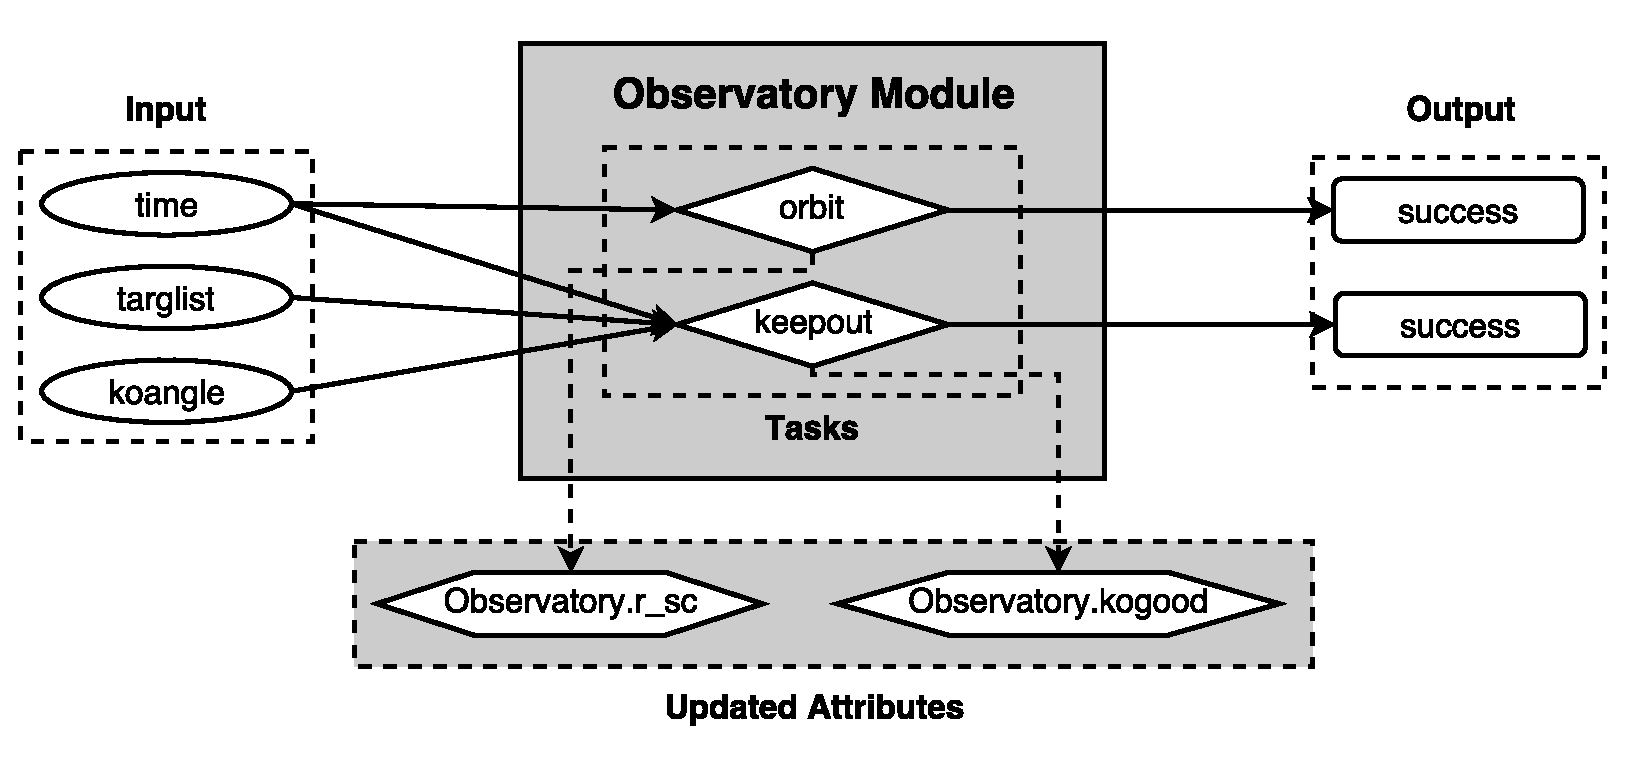
\includegraphics[width=0.9\textwidth]{observatory3}
        \end{tabular}
    \end{center}
    \caption{\label{fig:observatorymodule} Depiction of Observatory module methods including inputs, outputs, and updated attributes (see \S\ref{sec:orbittask} and \S\ref{sec:keepouttask}).}
\end{figure}

\label{sec:observatory}
\subsubsection{Observatory Object Attribute Initialization Input/Output Description}

\subsubsection*{Inputs}
\begin{itemize}
    \item
    \begin{description}
        \item[User specification] \hfill \\
        Information from simulation specification JSON file organized into a Python dictionary. If the below key: value pairs are missing from the dictionary, the Observatory object attributes will be assigned the default values listed.
        \begin{description}
            \item[settlingTime] \hfill \\
            Amount of time needed for observatory to settle after a repointing in $ days $. Default value is 1.
            \item[thrust] \hfill \\
            Occulter slew thrust in $ mN $. Default value is 450.
            \item[slewIsp] \hfill \\
            Occulter slew specific impulse in $ s $. Default value is 4160.
            \item[scMass] \hfill \\
            Occulter (maneuvering spacecraft) initial wet mass in $ kg $. Default value is 6000.
            \item[dryMass] \hfill \\
            Occulter (maneuvering spacecraft) dry mass in $ kg $. Default value is 3400.
            \item[coMass] \hfill \\
            Telescope (or non-maneuvering spacecraft) mass in $ kg $. Default value is 5800.
            \item[skIsp] \hfill \\
            Specific impulse for station keeping in $ s $. Default value is 220.
            \item[defburnPortion] \hfill \\
            Default burn portion for slewing. Default value is 0.05
            \item[spkpath] \hfill\\
            String with full path to SPK kernel file (only used if using jplephem for solar system body propagation - see \ref{sec:ssbPosTask}.
            \item[forceStaticEphem] \hfill \\
            Boolean, forcing use of static solar system ephemeris if set to True, even if jplephem module is present (see \ref{sec:ssbPosTask}).  Default value is False.
        \end{description}
    \end{description}
\end{itemize}

\subsubsection*{Attributes}
\begin{itemize}
    \item
    \begin{description}
        \item[settlingTime] \hfill \\
        Amount of time needed for observatory to settle after a repointing (astropy Quantity initially set in $ days $)
        \item[thrust] \hfill \\
        Occulter slew thrust (astropy Quantity initially set in $ mN $)
        \item[slewIsp] \hfill \\
        Occulter slew specific impulse (astropy Quantity initially set in $ s $)
        \item[scMass] \hfill \\
        Occulter (maneuvering spacecraft) initial wet mass (astropy Quantity initially set in $ kg $)
        \item[dryMass] \hfill \\
        Occulter (maneuvering spacecraft) dry mass (astropy Quantity initially set in $ kg $)
        \item[coMass] \hfill \\
        Telescope (or non-maneuvering spacecraft) mass (astropy Quantity initially set in $ kg $)
        \item[kogood] \hfill \\
        1D NumPy ndarray of Boolean values where True is a target unobstructed and observable in the keepout zone. Initialized to an empty array. This attribute is updated to the current mission time through the keepout method (see \ref{sec:keepouttask}).
        \item[r\_sc] \hfill \\
        Observatory orbit position in HE reference frame. Initialized to NumPy ndarray as numpy.array([0., 0., 0.]) and associated with astropy Quantity in $ km $. This attribute is updated to the orbital position of the observatory at the current mission time through the orbit method (see \ref{sec:orbittask}).
        \item[skIsp] \hfill \\
        Specific impulse for station keeping (astropy Quantity initially set in $ s $)
        \item[defburnPortion] \hfill \\
        Default burn portion for slewing
        \item[currentSep] \hfill \\
        Current occulter separation (astropy Quantity initially set in $ km $
        \item[flowRate] \hfill \\
        Slew flow rate derived from thrust and slewIsp (astropy Quantity initially set in $ kg/day $)
        
    \end{description}
\end{itemize}

\subsubsection{orbit Method Input/Output Description} \label{sec:orbittask}
The \verb+orbit+ method finds the heliocentric equatorial position vector of the observatory spacecraft.

\subsubsection*{Inputs}
\begin{itemize}
    \item
    \begin{description}
        \item[time] \hfill \\
        astropy \href{http://astropy.readthedocs.org/en/latest/time/index.html}{Time object} which may be \verb+TimeKeeping.currenttimeAbs+ from Time Keeping module see \ref{sec:currenttime} for definition
    \end{description}
\end{itemize}

\subsubsection*{Outputs}
\begin{itemize}
    \item
    \begin{description}
        \item[success] \hfill \\
        Boolean indicating if orbit was successfully calculated
    \end{description}
\end{itemize}

\subsubsection*{Updated Object Attributes}
\begin{itemize}
    \item
    \begin{description}
        \item[Observatory.r\_sc] \hfill \\
        Observatory orbit position in HE reference frame at current mission time (astropy Quantity defined in $ km $)
    \end{description}
\end{itemize}

\subsubsection{keepout Method Input/Output Description} \label{sec:keepouttask} 
The \verb+keepout+ method determines which stars in the target list are observable at the given input time.

\subsubsection*{Inputs}
\begin{itemize}
    \item
    \begin{description}
        \item[time] \hfill \\
        astropy Time object which may be \verb+TimeKeeping.currenttimeAbs+ (see \ref{sec:currenttime} for definition)
        \item[targlist] \hfill \\
        Instantiated Target List object from Target List module. See \ref{sec:targetlist} for definition of available attributes
        \item[koangle] \hfill \\
        Telescope keepout angle in degrees - \verb+OpticalSystem.telescopeKeepout+
    \end{description}
\end{itemize}

\subsubsection*{Outputs}
\begin{itemize}
    \item
    \begin{description}
        \item[success] \hfill \\
        Boolean indicating if orbit was successfully calculated
    \end{description}
\end{itemize}

\subsubsection*{Updated Object Attributes}
\begin{itemize}
    \item 
    \begin{description}
        \item[Observatory.kogood] \hfill \\
        1D NumPy ndarray of Boolean values for each target at given time where True is a target unobstructed in the keepout zone and False is a target unobservable due to obstructions in the keepout zone
    \end{description}
\end{itemize}

\subsubsection{solarSystem\_body\_position Method}\label{sec:ssbPosTask}
The \verb+solarSystem_body_position+ returns the position of any solar system body (Earth, Sun, Moon, etc.) at a given time in the common Heliocentric Equatorial frame.  The observatory prototype will attempt to load the jplephem module, and use a local SPK file for all propagations if available.  The SPK file is not packaged with the software but may be downloaded from JPL's website at: \url{http://naif.jpl.nasa.gov/pub/naif/generic_kernels/spk/planets/a_old_versions/}.  The location of the spk file is assumed to be in the Observatory directory but can be set by the \verb+spkpath+ input.  

If jplephem is not present, the Observatory prototype will load static ephemeris derived from Vallado (2004) and use those for propagation.  This behavior can be forced even when jplephem is available by setting the \verb+forceStaticEphem+ input to True.

\subsubsection*{Inputs}
\begin{itemize}
    \item
    \begin{description}
        \item[time] \hfill \\
        astropy Time object which may be \verb+TimeKeeping.currenttimeAbs+ (see \ref{sec:currenttime} for definition)
        \item[bodyname] \hfill \\
        String containing object name, capitalized by convention.
    \end{description}
\end{itemize}

\subsubsection*{Outputs}
\begin{itemize}
    \item
    \begin{description}
        \item[r\_body] \hfill \\
        (Quantity) heliocentric equatorial position vector (units of km)
    \end{description}
\end{itemize}

% TIME KEEPING 

\subsection{Time Keeping} \label{sec:time}
The Time Keeping module is responsible for keeping track of the current mission time.  It encodes only the mission start time, the mission duration, and the current time within a simulation.  All functions in all modules requiring knowledge of the current time call functions or access parameters implemented within the Time module.  Internal encoding of time is implemented as the time from mission start (measured in $ days $).  The Time Keeping module also provides functionality for converting between this time measure and standard measures such as Julian Day Number and UTC time.
  
The Time Keeping module contains the \verb+update_times+ and \verb+duty_cycle+ methods.  These  methods updates the mission time during a survey simulation.  The duty cycle determines when during the mission timeline the observatory is allowed to perform planet-finding operations.  The duty cycle function takes the current mission time as input and outputs the next available time when exoplanet observations may begin or resume, along with the duration of the observational period. The outputs of this method are used in the Survey Simulation module to determine when and how long exoplanet finding and characterization observations occur.  The inputs and updated attributes for the Time Keeping methods are depicted in \reffig{fig:timekeepingmodule}.

\begin{figure}[ht]
    \begin{center}
        \begin{tabular}{c}
             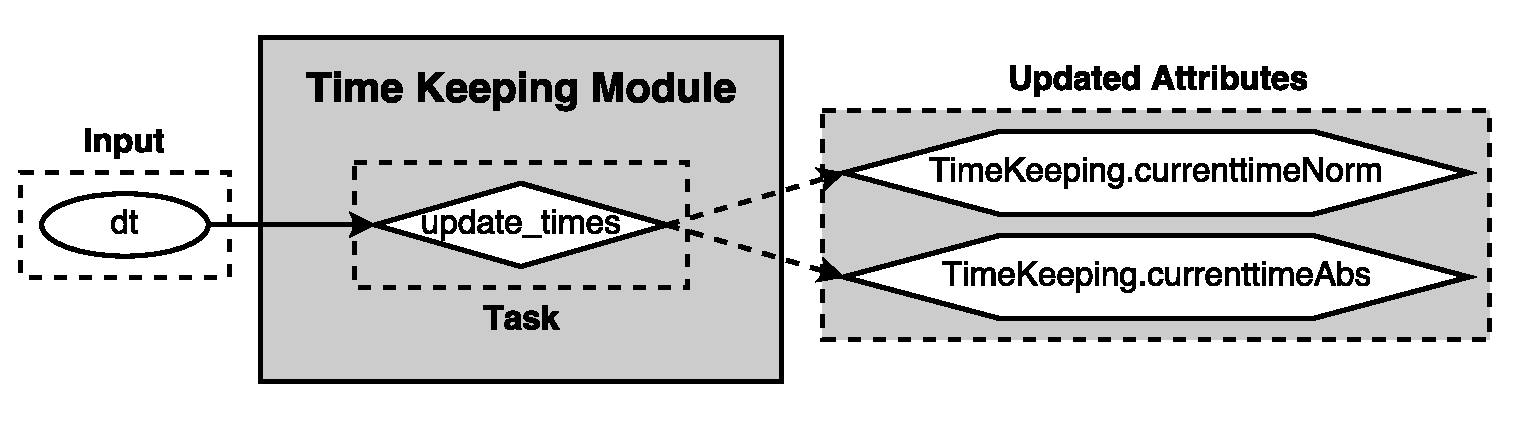
\includegraphics[width=\textwidth]{TimeKeepingTasks}
        \end{tabular}
    \end{center}
    \caption{\label{fig:timekeepingmodule} Depiction of Time Keeping module method including input and updated attributes (see \S\ref{sec:updatetimestask} and \S\ref{sec:dutycycletask}).}
\end{figure}

\subsubsection{Time Keeping Object Attribute Initialization Input/Output Description}

\subsubsection*{Inputs}
\begin{itemize}
    \item
     \begin{description}
            \item[missionStart] \hfill \\
            Mission start time in $ MJD $. Default value is 60634.
            \item[missionLife] \hfill \\
            Total length of mission in $ years $. Default value is 6.
            \item[extendedLife] \hfill \\
            Extended mission time in $ years $. Default value is 0.  Extended life typically differs from the primary mission in some way---most typically only revisits are allowed.
            \item[missionPortion] \hfill \\
            Portion of mission time devoted to planet-finding. Default value is 1/6.
        \end{description}
\end{itemize}

\subsubsection*{Attributes}
\begin{itemize}
    \item
    \begin{description}
        \item[missionStart] \hfill \\
        Mission start time (astropy Time object initially defined in $ MJD $)
        \item[missionLife] \hfill \\
        Mission lifetime (astropy Quantity initially set in $ years $)
        \item[extendedLife] \hfill \\
        Extended mission time (astropy Quantity initially set in $ years $)
        \item[missionPortion] \hfill \\
        Portion of mission time devoted to planet-finding
        \item[duration] \hfill \\
        Duration of planet-finding operations (astropy Quantity initially set in $ days $)
        \item[nexttimeAvail] \hfill \\
        Next time available for planet-finding (astropy Quantity initially set in $ days $)
        \item[currenttimeNorm] \hfill \\
        Current mission time normalized so that start date is 0 (astropy Quantity initially set in $ days $)
        \item[currenttimeAbs] \label{sec:currenttime}\hfill \\
        Current absolute mission time (astropy Time object initially defined in $ MJD $)
        \item[missionFinishNorm] \hfill \\
        Mission finish time (astropy Quantity initially set in $ days $)
        \item[missionFinishAbs] \hfill \\
        Mission completion date (astropy Time object initially defined in $ MJD $)
    \end{description}
\end{itemize}

\subsubsection{update\_times Method Input/Output Description} \label{sec:updatetimestask}
The \verb+update_times+ method updates the relevant mission times.

\subsubsection*{Inputs}
\begin{itemize}
    \item 
    \begin{description}
        \item[dt] \hfill \\
        Time increment (astropy Quantity with units of time)
    \end{description}
\end{itemize}

\subsubsection*{Updated Object Attributes}
\begin{itemize}
    \item 
    \begin{description}
        \item[TimeKeeping.currenttimeNorm] \hfill \\
        Current mission time normalized so that start date is 0 (astropy Quantity with units of time)
        \item[TimeKeeping.currenttimeAbs] \hfill \\
        Current absolute mission time (astropy Time object)
    \end{description}
\end{itemize}

\subsubsection{duty\_cycle Method Input/Output Description} \label{sec:dutycycletask}
The \verb+duty_cycle+ method calculates the next time that the observatory will be available for exoplanet science and returns this time and the maximum amount of time afterwards during which an exolanet observation can run (if capped).

\subsubsection*{Inputs}
\begin{itemize}
    \item 
    \begin{description}
        \item[currenttime] \hfill \\
        Current time in mission simulation (astropy Quantity with units of time often \verb+TimeKeeping.currenttimeNorm+)
    \end{description}
\end{itemize}

\subsubsection*{Outputs}
\begin{itemize}
    \item 
    \begin{description}
        \item[nexttime] \hfill \\
        Next available time for planet-finding (astropy Quantity with units of time)
    \end{description}
\end{itemize}

\subsubsection*{Updated Object Attributes}
\begin{itemize}
    \item 
    \begin{description}
        \item[TimeKeeping.nexttimeAvail] \hfill \\
        Next time available for planet-finding (astropy Quantity with units of time)
        \item[TimeKeeping.duration] \hfill \\
        Duration of planet-finding operations (astropy Quantity with units of time)
    \end{description}
\end{itemize}

% POST-PROCESSING

\subsection{Post-Processing}\label{sec:postprocessing}
The Post-Processing module encodes the effects of post-processing on the data gathered in a simulated observation, and the effects on the final contrast of the simulation.  The Post-Processing module is also responsible for determining whether a planet detection has occurred for a given observation, returning one of four possible states---true positive (real detection), false positive (false alarm), true negative (no detection when no planet is present) and false negative (missed detection).  These can be generated based solely on statistical modeling or by processing simulated images.

The Post-Processing module contains the \verb+det_occur+ task.  This task determines if a planet detection occurs for a given observation.  The inputs and outputs for this task are depicted in \reffig{fig:postprocessingmodule}.

\begin{figure}[ht]
    \begin{center}
        \begin{tabular}{c}
             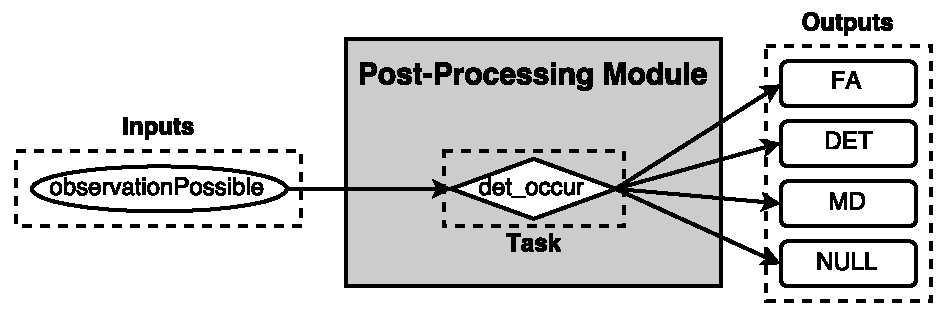
\includegraphics[width=0.8\textwidth]{PostTasks}
        \end{tabular}
    \end{center}
    \caption{\label{fig:postprocessingmodule} Depiction of Post-Processing module task including inputs and outputs (see \S\ref{sec:detoccurtask}).}
\end{figure}

\subsubsection{Post-Processing Object Attribute Initialization Input/Output Description}
\subsubsection*{Inputs}
\begin{itemize}
    \item 
    \begin{description}
          \item[FAP] \hfill \\
            Detection false alarm probability. Default value is $3 \times 10^{-5}$.
            \item[MDP] \hfill \\
            Missed detection probability. Default value is $10^{-3}$.
            \item[ppFact] \hfill \\
            Post-processing contrast factor, between 0 and 1. Default value is 1.
            \item[SNimag] \hfill \\
            Signal to Noise Ratio threshold for imaging/detection. Default value is 5.
            \item[SNchar] \hfill \\
            Signal to Noise Ratio threshold for characterization. Default value is 11.
        \end{description}
\end{itemize}

\subsubsection*{Attributes}
\begin{itemize}
    \item 
    \begin{description}
        \item[FAP] \hfill \\
        Detection false alarm probability
        \item[MDP] \hfill \\
        Missed detection probability
    \end{description}
\end{itemize}

\subsubsection{det\_occur Method Input/Output Description} \label{sec:detoccurtask}
The \verb+det_occur+ method determines if a planet detection has occurred.

\subsubsection*{Inputs}
\begin{itemize}
    \item 
    \begin{description}
        \item[observationPossible] \hfill \\
        1D NumPy ndarray of booleans signifying if a planet in the system being observed is observable
    \end{description}
\end{itemize}

\subsubsection*{Outputs}
\begin{itemize}
    \item 
    \begin{description}
        \item[FA] \hfill \\
        Boolean where True means False Alarm
        \item[DET] \hfill \\
        Boolean where True means DETection
        \item[MD] \hfill \\
        Boolean where True means Missed Detection
        \item[NULL] \hfill \\
        Boolean where True means Null Detection
    \end{description}
\end{itemize}

%%%%%%%%%%%%%%%%%%%%%%%%%%%%%%%%%%%%%%%%%%%%%%%%%%%%%%%%%%%%%%%%%%%%%%%%%
% SIMULATION MODULES
%%%%%%%%%%%%%%%%%%%%%%%%%%%%%%%%%%%%%%%%%%%%%%%%%%%%%%%%%%%%%%%%%%%%%%%%%

\section{Simulation Modules}
The simulation modules include Completeness, Target List, Simulated Universe, Survey Simulation and Survey Ensemble. These modules perform methods which require inputs from one or more input modules as well as calling function implementations in other simulation modules.

% COMPLETENESS

\subsection{Completeness}\label{sec:completeness}
The Completeness module takes in information from the Planet Population module to determine initial completeness and update completeness values for target list stars when called upon.

The Completeness module contains the following methods: \verb+target_completeness+ and \verb+completeness_update+. \verb+target_completeness+ generates initial completeness values for each star in the target list (see \S\ref{sec:targetcompletenesstask}). \verb+completeness_update+ updates the completeness values following an observation (see \S\ref{sec:completenessupdatetask}).

\subsubsection{Completeness Object Attribute Initialization Input/Output Description}

\subsubsection*{Input}
\begin{itemize}
    \item 
    \begin{description}
        \item[minComp] \hfill \\
            Minimum completeness value for inclusion in target list.  Defaults to 0.1.
    \end{description}
\end{itemize}

\subsubsection*{Attributes}
\begin{itemize}
    \item 
    \begin{description}
        \item[PlanetPopulation] \hfill \\
        Planet Population module object (see \ref{sec:planetpopulation})
        \item[minComp] \hfill \\
        Minimum completeness value for inclusion in target list. 
    \end{description}
\end{itemize}

\subsubsection{target\_completeness Method Input/Output Description}
\label{sec:targetcompletenesstask}
The \verb+target_completeness+ method generates completeness values for each star in the target list.

\subsubsection*{Inputs}
\begin{itemize}
    \item 
    \begin{description}
        \item[targlist] \hfill \\
        Instantiated Target List object from Target List module see \S\ref{sec:targetlist} for definition of functionality and attributes
    \end{description}
\end{itemize}

\subsubsection*{Outputs}
\begin{itemize}
    \item 
    \begin{description}
        \item[comp0] \hfill \\
        1D NumPy ndarray containing completeness values for each star in the target list
    \end{description}
\end{itemize}

\subsubsection{completeness\_update Method Input/Output Description}
\label{sec:completenessupdatetask}
The \verb+completeness_update+ method updates the completeness values for each star in the target list following an observation.

\subsubsection*{Inputs}
\begin{itemize}
    \item 
    \begin{description}
        \item[s\_ind] \hfill \\
        index of star in target list just observed
        \item[targlist] \hfill \\
        Instantiated Target List object from Target List module see \S\ref{sec:targetlist} for definition of functionality and attributes
        \item[obsbegin] \hfill \\
        Mission time when the observation of \verb+s_ind+ began (astropy Quantity with units of time)
        \item[obsend] \hfill \\
        Mission time when the observation of \verb+s_ind+ ended (astropy Quantity with units of time)
        \item[nexttime] \hfill \\
        Mission time of next observational period (astropy Quantity with units of time)
    \end{description}
\end{itemize}

\subsubsection*{Output}
\begin{itemize}
    \item 
    \begin{description}
        \item[comp0] \hfill \\
        1D NumPy ndarray of updated completeness values for each star in the target list
    \end{description}
\end{itemize}

% TARGET LIST

\subsection{Target List}
The Target List module takes in information from the Optical System, Star Catalog, Planet Population, and Observatory input modules and Completeness simulation module to generate the target list for the simulated survey.  This list can either contain all of the targets where a planet with specified parameter ranges could be observed or a list of pre-determined targets such as in the case of a mission which only seeks to observe stars where planets are known to exist from previous surveys.  The final target list encodes all of the same information as is provided by the Star Catalog module.

\label{sec:targetlist}
\subsubsection{Target List Object Attribute Initialization Input/Output Description}
\subsubsection*{Inputs}
\begin{itemize}
    \item 
    \begin{description}
        \item[User specification] \hfill \\
        Information from simulation specification JSON file organized into a Python dictionary. If key: value pairs are missing from the dictionary, the Target List object attributes will be assigned the default values.
        \item[StarCatalog] \hfill \\
        Instance of Star Catalog module (see \ref{sec:starcatalog})
        \item[keepStarCatalog] (bool) \hfill \\
        Boolean representing whether to delete the star catalog object after the target list is assembled (defaults to False).  If True, object reference will be available from TargetList object.
        \item[OpticalSystem] \hfill \\
        Instance of Optical System module (see \ref{sec:opticalsystem})
        \item[PlanetPopulation] \hfill \\
        Instance of Planet Population module (see \ref{sec:planetpopulation})
        \item[ZodiacalLight] \hfill \\
        Instance of Zodiacal Light module (see \ref{sec:zodiacallight})
        \item[Completeness] \hfill \\
        Instance of Completeness module (see \ref{sec:completeness})
    \end{description}
\end{itemize}

\subsubsection*{Attributes}
\begin{itemize}
    \item 
    \begin{description}
        \item[(StarCatalog values)] \hfill \\
        Mission specific filtered star catalog values from Star Catalog module (see \ref{sec:starcatalog})
        \item[OpticalSystem] \hfill \\
        Instance of Optical System module (see \ref{sec:opticalsystem})
        \item[PlanetPopulation] \hfill \\
        Instance of Planet Population module (see \ref{sec:planetpopulation})
        \item[ZodiacalLight] \hfill \\
        Instance of Zodiacal Light module (see \ref{sec:zodiacallight})
        \item[Completeness] \hfill \\
        Instance of Completeness module (see \ref{sec:completeness})
        \item[maxintTime] \hfill \\
        1D NumPy ndarray of maximum integration time for each target star found from \verb+OpticalSystem.calc_maxintTime+ \S\ref{sec:calcmaxintTimetask} (astropy Quantity with units of $days$)
        \item[comp0] \hfill \\
        1D NumPy ndarray of completeness value for each target star found from \verb+Completeness.target_completeness+ \S\ref{sec:targetcompletenesstask}
        \item[MsEst] \hfill \\
        Approximate stellar mass in $ M_{sun} $
        \item[MsTrue] \hfill \\
        Stellar mass with an error component included in $ M_{sun} $
        \item[nStars] \hfill \\
        Number of target stars
    \end{description}
\end{itemize}

% SIMULATED UNIVERSE 

\subsection{Simulated Universe} \label{sec:simulateduniverse}
The Simulated Universe module instantiate the Target List simulation module and creates a synthetic universe by populating planetary systems about some or all of the stars in the target list.  For each target, a planetary system is generated based on the statistics encoded in the Planet Population module, so that the overall planet occurrence and multiplicity rates are consistent with the provided distribution functions.  Physical parameters for each planet are similarly sampled from the input density functions (or calculated via the Planet physical model).  All planetary orbital and physical parameters are encoded as arrays of values, with an indexing array that maps planets to the stars in the target list. 

The Simulated Universe module contains the following methods: 
\begin{itemize}
\item[] \verb+planet_to_star+
\item[]  \verb+planet_pos_vel+
\item[]  \verb+prop_system+
\item[]  \verb+get_current_WA+
\end{itemize}
 \verb+planet_pos_vel+ finds initial position and velocity vectors for each planet (see \S\ref{sec:planetposveltask}).  \verb+prop_system+ propagates planet position and velocity vectors in time (see \S\ref{sec:propsystemtask}).  All planetary parameters are generated in the constructor via calls to the appropriate value generating functions in the planet population module.

%\begin{figure}[ht]
%    \begin{center}
%        \begin{tabular}{c}
%             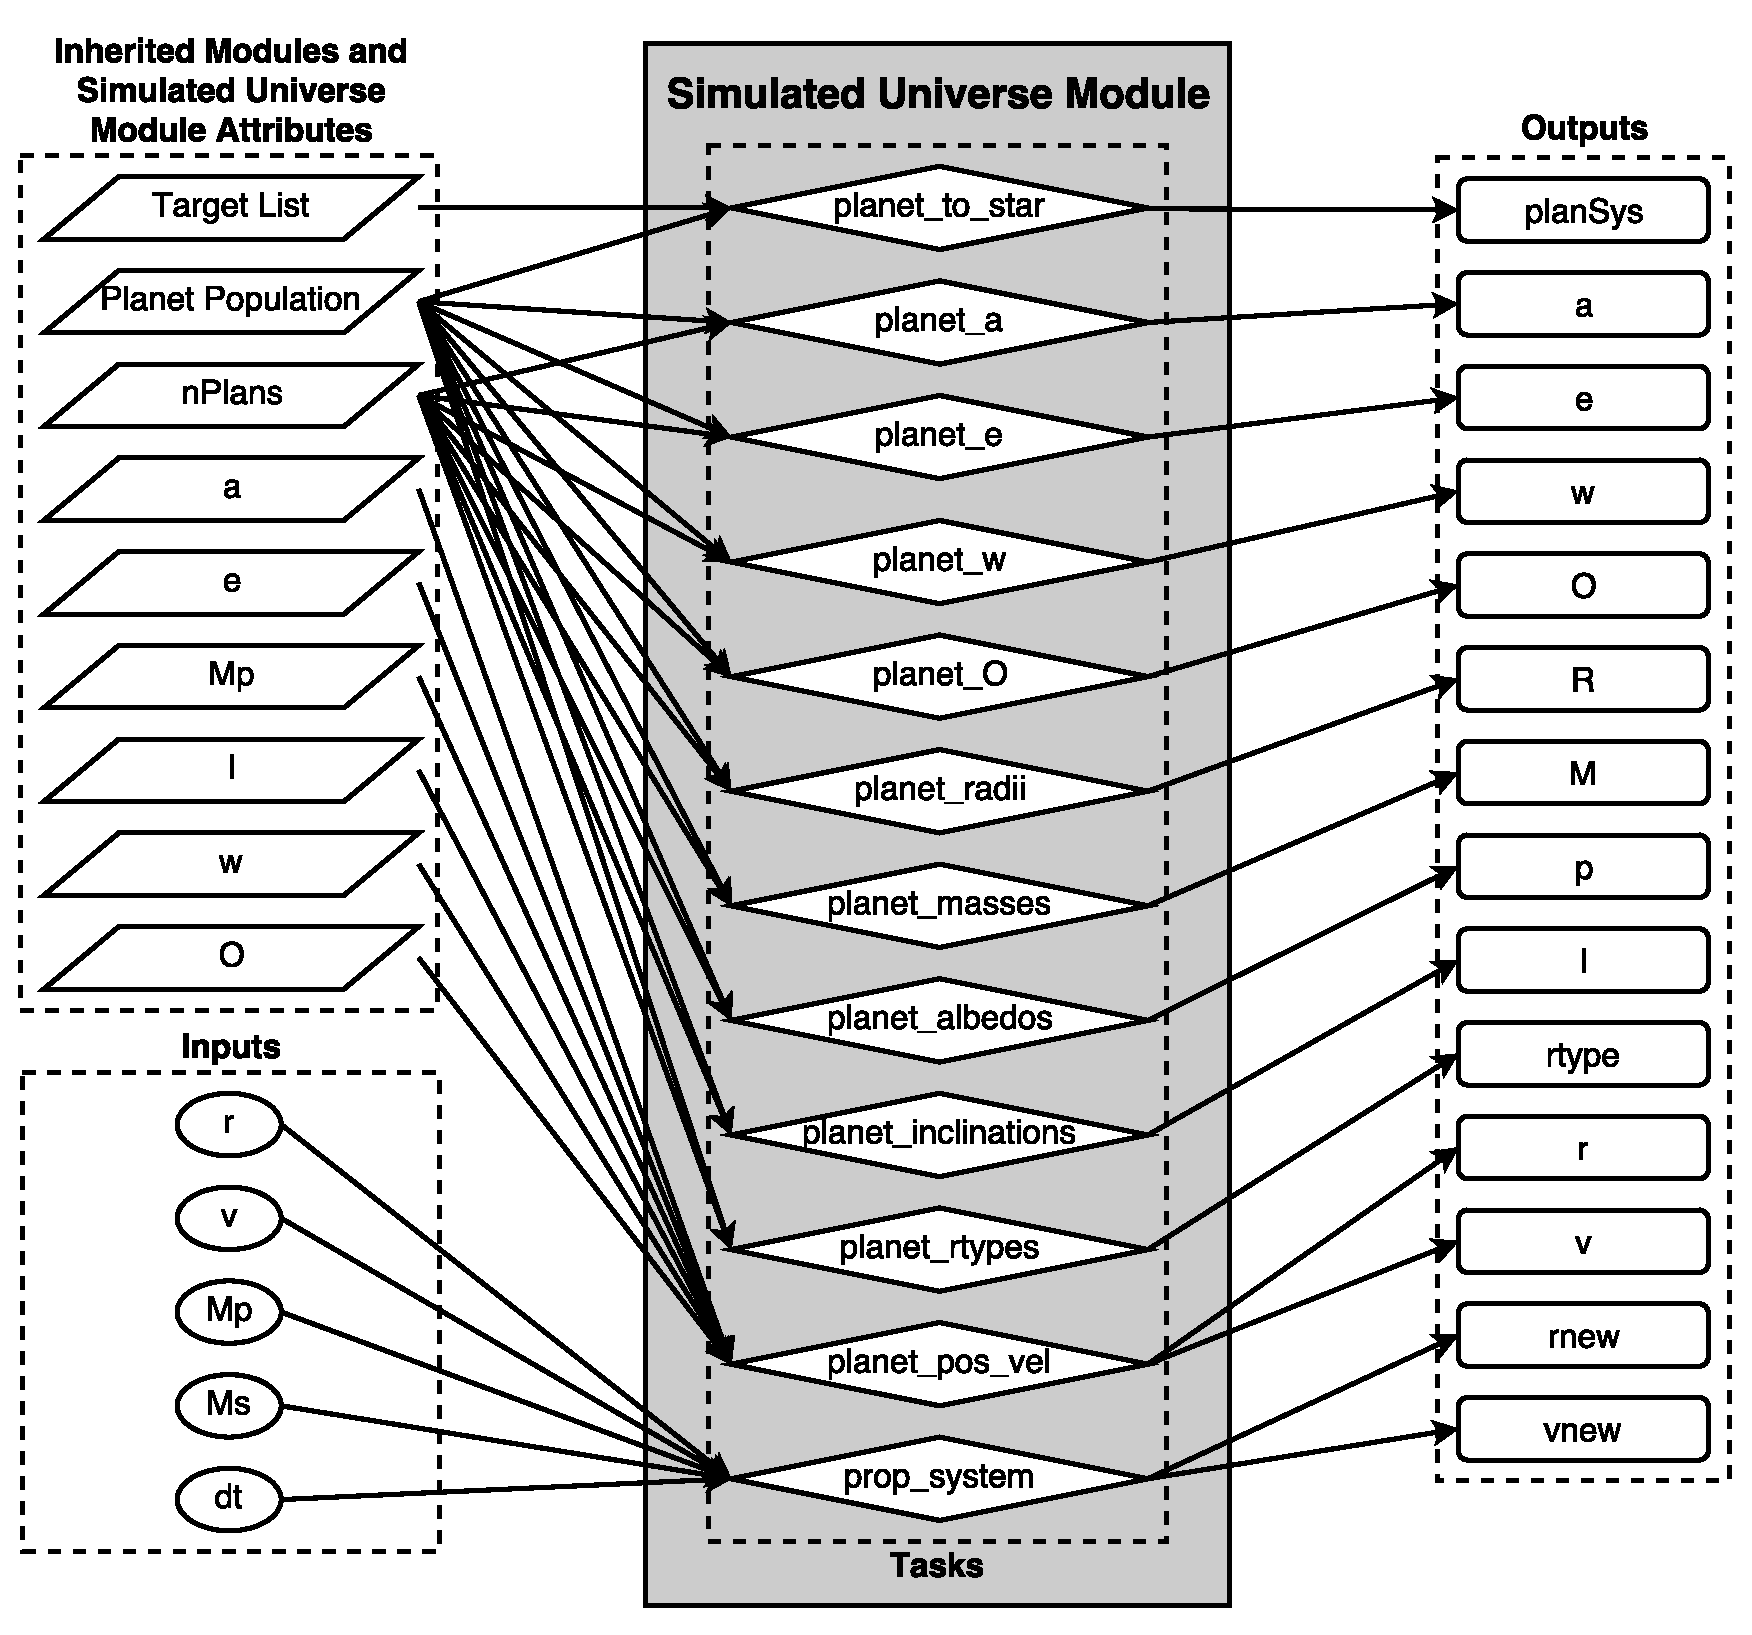
\includegraphics[width=\textwidth]{SimulatedUniverseTasks}
%        \end{tabular}
%    \end{center}
%    \caption{\label{fig:simulateduniversemodule} Depiction of Simulated Universe module methods including inputs and outputs (see \ref{sec:planettostartask}, \ref{sec:planetatask}, \ref{sec:planetetask}, \ref{sec:planetwtask}, \ref{sec:planetOtask}, \ref{sec:planetmassestask}, \ref{sec:planetradiitask}, \ref{sec:planetposveltask}, \ref{sec:planetalbedostask}, \ref{sec:planetinclinationstask}, and \ref{sec:propsystemtask}).}
%\end{figure}

\subsubsection{Attributes}
\begin{itemize}
    \item
    \begin{description}
        \item[OpticalSystem] \hfill \\
        Instance of Optical System module (see \ref{sec:opticalsystem})
        \item[PlanetPopulation] \hfill \\
        Instance of Planet Population module (see \ref{sec:planetpopulation})
        \item[ZodiacalLight] \hfill \\
        Instance of Zodiacal Light module (see \ref{sec:zodiacallight})
        \item[Completeness] \hfill \\
        Instance of Completeness module (see \ref{sec:completeness})
        \item[TargetList] \hfill \\
        Instance of Target List module (see \ref{sec:targetlist})
        \item[PlanetPhysicalModel] \hfill \\
        Instance of Planet Physical Model module (see \ref{sec:planetphysicalmodel})
        \item[planInds] \hfill \\
        1D NumPy ndarray containing indices (referenced to exoplanet list) mapping each planet to its star determined from \verb+planet_to_star()+ \S\ref{sec:planettostartask}
        \item[nPlans] \hfill \\
        Number of planets (determined from \verb+len(SimulatedUniverse.planInds)+)
        \item[sysInds] \hfill \\
        1D NumPy ndarray containing indices (referenced to target star list) of target stars with planets
        \item[a] \hfill \\
        Quantity array containing semi-major axis for each planet 
        \item[e] \hfill \\
        1D NumPy ndarray containing eccentricity values for each planet
        \item[w] \hfill \\
        Quantity array containing argument of perigee in degrees for each planet
        \item[O] \hfill \\
        Quantity array containing right ascension of the ascending node in degrees for each planet
        \item[Mp] \hfill \\
        Quantity array containing masses of each planet
        \item[Rp] \hfill \\
        Quantity array containing radii of each planet
        \item[r] \hfill \\
        Quantity array containing planet position vectors relative to host stars
        \item[v] \hfill \\
        Quantity array containing planet velocity vectors relative to host stars 
        \item[p] \hfill \\
        1D NumPy ndarray containing planet geometric albedos
        \item[I] \hfill \\
        Quantity array containing list of inclination of planetary systems in degrees 
        \item[fzodicurr] \hfill \\
        1D NumPy ndarray containing list of exozodi levels for systems with planets determined from \verb+ZodiacalLight.fzodi+ \S\ref{sec:fzoditask}
    \end{description}
\end{itemize}

\subsubsection{planet\_to\_star Method Input/Output Description} \label{sec:planettostartask}
The \verb+planet_to_star+ method determines how many planets belong to each star in the target list.  It returns a 1D NumPy ndarray containing the indices of the target star to which each planet belongs.  The length of the ndarray is the total number of planets in the simulated universe.

\subsubsection*{Inputs}
This method does not take any explicit inputs.  It uses the inherited Target List and Planet Population objects.

\subsubsection*{Updated Attributes}
\begin{itemize}
    \item 
    \begin{description}
        \item[planSys] \hfill \\
        1D NumPy ndarray containing the indices of each target star to which each planet (each element of the array) belongs
         \item[sysInds] \hfill \\
        1D NumPy ndarray containing the indices of only those target stars which have planets
    \end{description}
\end{itemize}

\subsubsection{planet\_pos\_vel Method Input/Output Description} \label{sec:planetposveltask}
The \verb+planet_pos_vel+ method assigns each planet an initial position and velocity vector with appropriate astropy Quantity units attached.

\subsubsection*{Inputs}
This method does not take any explicit inputs.  It uses the following attributes assigned before calling this method:
\begin{itemize}
    \item \verb+SimulatedUniverse.a+
    \item \verb+SimulatedUniverse.e+
    \item \verb+SimulatedUniverse.Mp+
    \item \verb+SimulatedUniverse.I+
    \item \verb+SimulatedUniverse.w+
    \item \verb+SimulatedUniverse.O+
\end{itemize}

\subsubsection*{Outputs}
\begin{itemize}
    \item 
    \begin{description}
        \item[r] \hfill \\
        NumPy ndarray containing initial position vector for each planet (astropy Quantity with default units of $ km $)
        \item[v] \hfill \\
        NumPy ndarray containing initial velocity vector for each planet (astropy Quantity with default units of $ km/s $)
    \end{description}
\end{itemize}

\subsubsection{prop\_system Method Input/Output Description} \label{sec:propsystemtask}
The \verb+prop_system+ method propagates planet state vectors (position and velocity) in time.

\subsubsection*{Inputs}
\begin{itemize}
    \item 
    \begin{description}
        \item[r] \hfill \\
        NumPy ndarray containing current planet position vectors relative to host star (astropy Quantity with units of distance)
        \item[v] \hfill \\
        NumPy ndarray containing current planet velocity vectors relative to host star (astropy Quantity with units of distance/time)
        \item[Mp] \hfill \\
        1D NumPy ndarray containing planet masses (astropy Quantity with units of mass)
        \item[Ms] \hfill \\
        1D NumPy ndarray containing target star mass in $ M_{sun} $
        \item[dt] \hfill \\
        Time increment to propagate system (astropy Quantity with units of time)
    \end{description}
\end{itemize}

\subsubsection*{Outputs}
\begin{itemize}
    \item 
    \begin{description}
        \item[rnew] \hfill \\
        NumPy ndarray of propagated position vectors relative to host star (astropy Quantity with units of distance)
        \item[vnew] \hfill \\
        NumPy ndarray of propagated velocity vectors relative to host star (astropy Quantity with units of distance/time)
    \end{description}
\end{itemize}

\subsubsection{get\_current\_WA Method Input/Output Description} \label{sec:getcurrentWAtask}
The \verb+get_current_WA+ method calculates the current working angles for planets specified by the given indices.

\subsubsection*{Inputs}
\begin{itemize}
    \item 
    \begin{description}
        \item[Inds] \hfill \\
        1D NumPy ndarray containing integer indices of the planets of interest
    \end{description}
\end{itemize}

\subsubsection*{Outputs}
\begin{itemize}
    \item 
    \begin{description}
        \item[wa] \hfill \\
        1D NumPy ndarray containing working angles (units of arcsecons)
    \end{description}
\end{itemize}

% SURVEY SIMULATION

\subsection{Survey Simulation} \label{sec:surveysim}
The Survey Simulation module takes as input instances of the Simulated Universe simulation module and the Time Keeping, and Post-Processing input modules. This is the module that performs a specific simulation based on all of the input parameters and models. This module returns the mission timeline - an ordered list of simulated observations of various targets on the target list along with their outcomes.  The output also includes an encoding of the final state of the simulated universe (so that a subsequent simulation can start from where a previous simulation left off) and the final state of the observatory definition (so that post-simulation analysis can determine the percentage of volatiles expended, and other engineering metrics).

Survey Simulation TASKS: 
\verb+run_sim()+ - perform survey simulation \S\ref{sec:runsimtask}

Survey Simulation SUBTASKS:
\verb+initial_target()+ - find initial target star \S\ref{sec:initialtargettask}

\verb+observation_detection(pInds, s_ind, DRM, planPosTime)+ - finds if planet detections are possible and returns relevant information \S\ref{sec:observationdetectiontask}\\
\verb+det_data(s, dMag, Ip, DRM, FA, DET, MD, s_ind, pInds, observationPossible, observed)+ - determines detection status \S\ref{sec:detdatatask}
\begin{verbatim}
observation_characterization(observationPossible, pInds, s_ind, spectra,\
	 					s, Ip, DRM, FA, t_int)
\end{verbatim} 
finds if characterizations are possible and returns relevant information \S\ref{sec:observationcharacterizationtask}\\
\verb+next_target(s_ind, revisit_list, extended_list, DRM)+ - find next target (scheduler) \S\ref{sec:nexttargettask}

\subsubsection{Survey Simulation Object Attribute Initialization Input/Output Description}
\subsubsection*{Inputs}
\begin{itemize}
    \item 
    \begin{description}
        \item[User specification] \hfill \\
        Information from simulation specification JSON file organized into a Python dictionary. If the below key: value pairs are missing from the dictionary, the Survey Simulation object attributes will be assigned the default values listed.
        \item[OpticalSystem] \hfill \\
        Instance of Optical System module inherited from Simulated Universe module (see \ref{sec:opticalsystem})
        \item[PlanetPopulation] \hfill \\
        Instance of Planet Population module inherited from Simulated Universe module (see \ref{sec:planetpopulation})
        \item[ZodiacalLight] \hfill \\
        Instance of Zodiacal Light module inherited from Simulated Universe module (see \ref{sec:zodiacallight})
        \item[Completeness] \hfill \\
        Instance of Completeness module inherited from Simulated Universe module (see \ref{sec:completeness})
        \item[TargetList] \hfill \\
        Instance of Target List module inherited from Simulated Universe module (see \ref{sec:targetlist})
        \item[PlanetPhysicalModel] \hfill \\
        Instance of Planet Physical Model module inherited from Simulated Universe module (see \ref{sec:planetphysicalmodel})
        \item[SimulatedUniverse] \hfill \\
        Instance of Simulated Universe module (see \ref{sec:simulateduniverse})
        \item[Observatory] \hfill \\
        Instance of Observatory module (see \ref{sec:observatory})
        \item[TimeKeeping] \hfill \\
        Instance of Time Keeping module (see \ref{sec:time})
        \item[PostProcessing] \hfill \\
        Instance of Post-Processing module (see \ref{sec:postprocessing})
    \end{description}
\end{itemize}

\subsubsection*{Attributes}
\begin{itemize}
    \item
    \begin{description}
        \item[OpticalSystem] \hfill \\
        Instance of Optical System module (see \ref{sec:opticalsystem})
        \item[PlanetPopulation] \hfill \\
        Instance of Planet Population module (see \ref{sec:planetpopulation})
        \item[ZodiacalLight] \hfill \\
        Instance of Zodiacal Light module (see \ref{sec:zodiacallight})
        \item[Completeness] \hfill \\
        Instance of Completeness module (see \ref{sec:completeness})
        \item[TargetList] \hfill \\
        Instance of Target List module (see \ref{sec:targetlist})
        \item[PlanetPhysicalModel] \hfill \\
        Instance of Planet Physical Model module (see \ref{sec:planetphysicalmodel})
        \item[SimulatedUniverse] \hfill \\
        Instance of Simulated Universe module (see \ref{sec:simulateduniverse})
        \item[Observatory] \hfill \\
        Instance of Observatory module (see \ref{sec:observatory})
        \item[TimeKeeping] \hfill \\
        Instance of Time Keeping module (see \ref{sec:time})
        \item[PostProcessing] \hfill \\
        Instance of Post-Processing module (see \ref{sec:postprocessing})
        \item[DRM] \hfill \\
        Contains the results of survey simulation
    \end{description}
\end{itemize}

\subsubsection{run\_sim Method Input/Output Description} \label{sec:runsimtask}
The \verb+run_sim+ method performs the survey simulation and populates the results in \verb+SurveySimulation.DRM+.

\subsubsection*{Inputs}
This method does not take any explicit inputs.  It uses the inherited modules to generate a survey simulation.

\subsubsection*{Updated Object Attributes}
\begin{itemize}
    \item 
    \begin{description}
        \item[SurveySimulation.DRM] \hfill \\
        Python list where each entry contains a dictionary of survey simulation results for each observation.  The dictionary may include the following key:value pairs (from the prototype):
        \begin{description}
            \item[target\_ind] \hfill \\
            Index of star in target list observed
            \item[arrival\_time] \hfill \\
            Days since mission start when observation begins
            \item[sc\_mass] \hfill \\
            Maneuvering spacecraft mass (if simulating an occulter system)
            \item[dF\_lateral] \hfill \\
            Lateral disturbance force on occulter in $ N $ if simulating an occulter system
            \item[dF\_axial] \hfill \\
            Axial disturbance force on occulter in $ N $ if simulating an occulter system
            \item[det\_dV] \hfill \\
            Detection station-keeping $\Delta$V in $ m/s $ if simulating an occulter system
            \item[det\_mass\_used] \hfill \\
            Detection station-keeping fuel mass used in $ kg $ if simulating an occulter system
            \item[det\_int\_time] \hfill \\
            Detection integration time in $ days $
            \item[det\_status] \hfill \\
            Integer or list where
            \begin{itemize}
                \item 1 = detection
                \item 0 = null detection
                \item -1 = missed detection
                \item -2 = false alarm
            \end{itemize}
            \item[det\_WA] \hfill \\
            Detection WA in $ mas $
            \item[det\_dMag] \hfill \\
            Detection $ \Delta $mag
            \item[char\_1\_time] \hfill \\
            Characterization integration time in $ days $
            \item[char\_1\_dV] \hfill \\
            Characterization station-keeping $\Delta$V in $ m/s $ if simulating an occulter system
            \item[char\_1\_mass\_used] \hfill \\
            Characterization station-keeping fuel mass used in $ kg $ if simulating an occulter system
            \item[char\_1\_success] \hfill \\
            Characterization success where value which may be:
            \begin{itemize}
                \item 1 - successfull characterization
                \item effective wavelength found during characterization in $ nm $
            \end{itemize}
            \item[slew\_time] \hfill \\
            Slew time to next target in $ days $ if simulating an occulter system
            \item[slew\_dV] \hfill \\
            Slew $\Delta$V in $ m/s $ if simulating an occulter system
            \item[slew\_mass\_used] \hfill \\
            Slew fuel mass used in $ kg $ if simulating an occulter system
            \item[slew\_angle] \hfill \\
            Slew angle to next target in $ rad $
        \end{description}
    \end{description}
\end{itemize}

\subsubsection{initial\_target Sub-task Input/Output Description} \label{sec:initialtargettask}
The \verb+initial_target+ sub-task is called from the \verb+run_sim+ method to determine the index of the initial target star in the target list.

\subsubsection*{Inputs}
This sub-task does not take any explicit inputs.  It may use any of the inherited modules to generate the initial target star index.

\subsubsection*{Outputs}
\begin{itemize}
    \item 
    \begin{description}
        \item[s\_ind] \hfill \\
        Index of the initial target star
    \end{description}
\end{itemize}

\subsubsection{observation\_detection Sub-task Input/Output Description} \label{sec:observationdetectiontask}
The \verb+observation_detection+ sub-task is called from the \verb+run_sim+ task to determine if planets may be detected and calculate information needed later in the simulation.

\subsubsection*{Inputs}
\begin{itemize}
    \item 
    \begin{description}
        \item[pInds] \hfill \\
        1D NumPy ndarray of indices of planets belonging to the target star (used to get relevant attributes from the \verb+SimulatedUniverse+ module)
        \item[s\_ind] \hfill \\
        Index of target star in target list
        \item[DRM] \hfill \\
        Python dictionary containing survey simulation results of current observation as key:value pairs
        \item[planPosTime] \hfill \\
        1D NumPy ndarray containing the times at which the planet positions and velocities contained in \verb+SimulatedUniverse.r+ and \verb+SimulatedUniverse.v+ are current (astropy Quantity with units of time)
    \end{description}
\end{itemize}

\subsubsection*{Outputs}
\begin{itemize}
    \item 
    \begin{description}
        \item[observationPossible] \hfill \\
        1D NumPy ndarray (length is number of planets in the system under observation) containing boolean values where True is an observable planet
        \item[t\_int] \hfill \\
        Integration time (astropy Quantity with units of time)
        \item[DRM] \hfill \\
        Python dictionary containing survey simulation results of current observation as key:value pairs
        \item[s] \hfill \\
        1D NumPy ndarray (length is number of planets in the system under observation) containing apparent separation of planets (astropy Quantity with units of distance)
        \item[dMag] \hfill \\
        1D NumPy ndarray (length is number of planets in the system under observation) containing $ \Delta $mag for each planet
        \item[Ip] \hfill \\
        1D NumPy ndarray (length is number of planets in the system under observation) containing irradiance (astropy Quantity with units of $ \frac{1}{m^2 \cdot nm \cdot s} $)
    \end{description}
\end{itemize}

\subsubsection{det\_data Sub-task Input/Output Description} \label{sec:detdatatask}
The \verb+det_data+ sub-task is called from the \verb+run_sim+ task to assign a detection status to the dictionary of current observation results.

\subsubsection*{Inputs}
\begin{itemize}
    \item 
    \begin{description}
        \item[s] \hfill \\
        1D NumPy array (length is number of planets in the system under observation) containing apparent separation of planets (astropy Quantity with units of distance)
        \item[dMag] \hfill \\
        1D NumPy ndarray (length is number of planets in the system under observation) containing $ \Delta $mag for each planet
        \item[Ip] \hfill
        1D NumPy ndarray (length is number of planets in the system under observation) containing irradiance (astropy Quantity with units of $ \frac{1}{m^2 \cdot nm \cdot s} $)
        \item[DRM] \hfill \\
        Python dictionary containing survey simulation results of current observation as key:value pairs
        \item[FA] \hfill \\
        Boolean where True is False Alarm
        \item[DET] \hfill \\
        Boolean where True is DETection
        \item[MD] \hfill \\
        Boolean where True is Missed Detection
        \item[s\_ind] \hfill \\
        Index of target star in target list
        \item[pInds] \hfill \\
        1D NumPy ndarray of indices of planets belonging to the target star (used to get relevant attributes from the \verb+SimulatedUniverse+ module)
        \item[observationPossible] \hfill \\
        1D NumPy ndarray (length is number of planets in the system under observation) containing boolean values where True is an observable planet
        \item[observed] \hfill \\
        1D NumPy ndarray which contains the number of observations for each planet in the simulated universe
    \end{description}
\end{itemize}

\subsubsection*{Outputs}
\begin{itemize}
    \item 
    \begin{description}
        \item[s] \hfill \\
        1D NumPy array (length is number of planets in the system under observation) containing apparent separation of planets (astropy Quantity with units of distance)
        \item[dMag] \hfill \\
        1D NumPy ndarray (length is number of planets in the system under observation) containing $ \Delta $mag for each planet
        \item[Ip] \hfill \\
        1D NumPy ndarray (length is number of planets in the system under observation) containing irradiance (astropy Quantity with units of $ \frac{1}{m^2 \cdot nm \cdot s} $)
        \item[DRM] \hfill \\
        Python dictionary containing survey simulation results of current observation as key:value pairs
        \item[observed] \hfill \\
        1D NumPy ndarray which contains the number of observations for each planet in the simulated universe
    \end{description}
\end{itemize}

\subsubsection{observation\_characterization Sub-task Input/Output Description} \label{sec:observationcharacterizationtask}
The \verb+observation_characterization+ sub-task is called by the \verb+run_sim+ task to determine if characterizations are to be performed and calculate relevant characterization information to be used later in the observation simulation.

\subsubsection*{Inputs}
\begin{itemize}
    \item 
    \begin{description}
        \item[observationPossible] \hfill \\
        1D NumPy ndarray (length is number of planets in the system under observation) containing boolean values where True is an observable planet
        \item[pInds] \hfill \\
        1D NumPy ndarray of indices of planets belonging to the target star (used to get relevant attributes from the \verb+SimulatedUniverse+ module)
        \item[s\_ind] \hfill \\
        Index of target star in target list
        \item[spectra] \hfill \\
        NumPy ndarray where 1 denotes spectra for a planet that has been captured, 0 denotes spectra for a planet that has not been captured
        \item[s] \hfill \\
        1D NumPy array (length is number of planets in the system under observation) containing apparent separation of planets (astropy Quantity with units of distance)
        \item[Ip] \hfill \\
        1D NumPy ndarray (length is number of planets in the system under observation) containing irradiance (astropy Quantity with units of $ \frac{1}{m^2 \cdot nm \cdot s} $)
        \item[DRM] \hfill \\
        Python dictionary containing survey simulation results of current observation as key:value pairs
        \item[FA] \hfill \\
        Boolean where True is False Alarm
        \item[t\_int] \hfill \\
        Integration time (astropy Quantity with units of time)
    \end{description}
\end{itemize}

\subsubsection*{Outputs}
\begin{itemize}
    \item 
    \begin{description}
        \item[DRM] \hfill \\
        Python dictionary containing survey simulation results of current observation as key:value pairs
        \item[FA] \hfill \\
        Boolean where True is False Alarm
        \item[spectra] \hfill \\
        NumPy ndarray where 1 denotes spectra for a planet that has been captured, 0 denotes spectra for a planet that has not been captured
    \end{description}
\end{itemize}

\subsubsection{next\_target Sub-task Input/Output Description} \label{sec:nexttargettask}
The \verb+next_target+ sub-task is called from the \verb+run_sim+ task to determine the index of the next star from the target list for observation.

\subsubsection*{Inputs}
\begin{itemize}
    \item 
    \begin{description}
        \item[s\_ind] \hfill \\
        Index of current star from the target list
        \item[targlist] \hfill \\
        Target List module (see \ref{sec:targetlist})
        \item[revisit\_list] \hfill \\
        NumPy ndarray containing index of target star and time in $ days $ of target stars from the target list to revisit
        \item[extended\_list] \hfill \\
        1D NumPy ndarray containing the indices of stars in the target list to consider if in extended mission time
        \item[DRM] \hfill \\
        Python dictionary containing survey simulation results of current observation as key:value pairs
    \end{description}
\end{itemize}

\subsubsection*{Outputs}
\begin{itemize}
    \item 
    \begin{description}
        \item[new\_s\_ind] \hfill \\
        Index of next target star in the target list
        \item[DRM] \hfill \\
        Python dictionary containing survey simulation results of current observation as key:value pairs
    \end{description}
\end{itemize}

% SURVEY ENSEMBLE NEEDS UPDATING

\subsection{Survey Ensemble}
The Survey Ensemble module's only task is to run multiple simulations.  While the implementation of this module is not at all dependent on a particular mission design, it can vary to take advantage of available parallel-processing resources.  As the generation of a survey ensemble is an embarrassingly parallel task---every survey simulation is fully independent and can be run as a completely separate process---significant gains in execution time can be achieved with parallelization.  The baseline implementation of this module contains a simple looping function that executes the desired number of simulations sequentially, as well as a locally parallelized version based on IPython Parallel.

Depending on the local setup, the Survey Ensemble implementation could also potentially save time by cloning survey module objects and reinitializing only those sub-modules that have stochastic elements (i.e., the simulated universe).

Another possible implementation variation is to use the Survey Ensemble module to conduct investigations of the effects of varying any normally static parameter.  This could be done, for example, to explore the impact on yield in cases where the non-coronagraph system throughput, or elements of the propulsion system, are mischaracterized prior to launch.  This SE module implementation would overwrite the parameter of interest given in the input specification for every individual survey executed, and saving the true value of the parameter used along with the simulation output.

\end{document}
